\chapter{Related problems}
\label{sec:other_problems}

The primary motivation for using a mathematical formulation as the solving method is \emph{flexibility}.
The possibility of adapting a formulation for other problems or variants often stays theoretical and occasionally is materialised and empirically examined.
This chapter describes the changes necessary to adapt the BBA formulation to the Guillotine 2D version of three other problems from the cutting and packing literature.
It also presents empirical results of these adaptations over suitable datasets.
As far as the author knows, the closest work to ours regarding this aspect is~\citet{bezerra:2020} which adapts two MILP models from the literature to the `two-dimensional level strip packing problem' (as they call it).

\section{Problems definitions}

The three related problems this chapter considers are the Guillotine 2D version of the Multiple Knapsack Problem (MKP), the Orthogonal Packing Problem (OPP), and the Cutting Stock Problem (CSP).
The CSP is closely related to the Bin Packing Problem, BPP; the distinctions are discussed further ahead.
Both the G2MKP and the G2CSP consider multiple original plates and, therefore, have homogeneous and heterogeneous variants.
The G2MKP (or the G2CSP) is homogeneous if its multiple original plates share the same dimensions.
It is heterogeneous if the original plates may come in distinct sizes (which may have a different cost associated with each).
 This work covers only the adaptation to the homogeneous variant, which is the simpler one of the two options.

\emph{The (homogeneous) G2MKP} is the generalization of the G2KP in which, instead of having a single copy of the original plate available, there are \(m\)~copies of the original plate available; nevertheless, both G2KP and the homogeneous G2MKP have only one original plate \emph{type}, i.e., all the \(m\) original plate copies share the same dimensions (\(L\)x\(W\)).
G2MKP instances only differ from G2KP instances by this extra parameter~(\(m\)).
Adaptation of G2KP instances to the G2MKP by an unmindful increase of \(m\) may lead to trivial instances because it may become trivial to pack every piece.

\emph{The G2OPP} is the decision problem that inquires if a specific set of pieces can be packed into a plate of specific dimensions using only guillotine cuts.
Compared to G2KP, the main differences of G2OPP instances are that (i) there are no piece profits, (ii) the piece demand is not an upper bound, but a lower bound, and (iii) any instance with a summed piece area greater than the original plate area is trivially false and, therefore, not interesting.
Piece profits may be dropped, and the demand may be reinterpreted, but the third distinction makes most instances of the G2KP uninteresting for the G2OPP.

\emph{The (homogeneous) G2CSP} consists of minimizing the number of copies of the single original plate type while packing every copy of every piece type.
The main differences between G2CSP and G2KP instances are that, in G2CSP instances: (i) there are no piece profits, (ii) the piece demand is not an upper bound but a lower bound, and (iii) trivial instances usually have the summed area of all pieces slightly larger than the closest multiple of the original plate area; such trait is not uncommon for G2KP instances.
For example, if the area of the original plate type is 100, and the summed area of all pieces is 301, then there is a good chance of the optimal solution value to be 4 (i.e., the trivial area lower bound).
The optimal solution cannot be less than four original plates. To need five or more original plates, the piece multiset would need to be designed to cause an uncommonly high waste ratio (i.e., greater than \(25\%\)).
Moreover, there will probably exist not only one but many (nonsymmetrical) solutions able to pack all pieces into four original plates. This variety will make it easier for the solver to find an upper bound that matches the trivial lower bound.

Neither G2MKP nor G2CSP can be solved exactly by successively applying G2KP to the multiset of pieces yet unpacked.
\Cref{fig:related_problems_diagram} shows a proof of this statement and helps to visualise the differences between these three problems.
For the G2OPP, the example instance is trivially false.

\begin{figure}[h]
  \caption{Visual proof G2KP cannot be iteratively used to solve G2MKP/G2CSP.}
  \center
  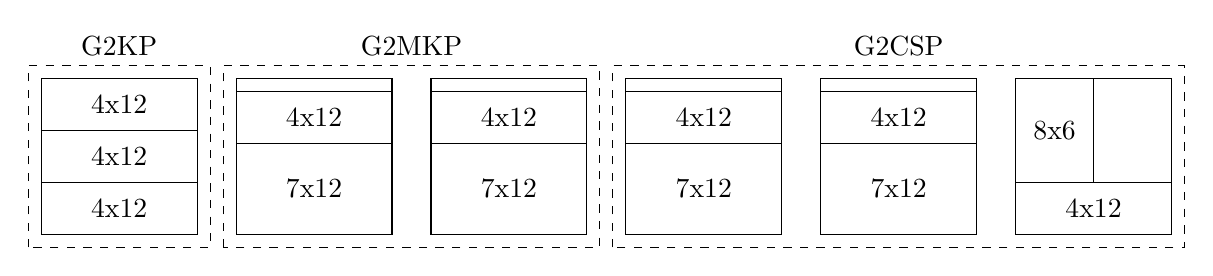
\begin{tikzpicture}[scale=0.165]
\def\piececolor{gray!20}
\def\labelxshift{12.5}
\def\labelyshift{0}
\def\labelfontsize{\normalsize}

\begin{scope}[shift={(0, 0)}]
\begin{scope}[shift={(0, 0)}]

\draw [dashed] (-1, -1) rectangle +(14, 14);
\path (-1, 13)  -- +(14, 0) node [above, midway, align=center] {\labelfontsize G2KP};

\draw (0, 0) rectangle +(12, 4) node[midway] {\labelfontsize 4x12};
\draw (0, 4) rectangle +(12, 4) node[midway] {\labelfontsize 4x12};
\draw (0, 8) rectangle +(12, 4) node[midway] {\labelfontsize 4x12};

\draw (0,0) rectangle +(12, 12);

\end{scope}

\begin{scope}[shift={(15, 0)}]

\draw [dashed] (-1, -1) rectangle +(29, 14);
\path (-1, 13) -- +(29, 0) node [above, midway, align=center] {\labelfontsize G2MKP};

\begin{scope}[shift={(0, 0)}]
\draw (0, 0) rectangle +(12, 7) node[midway] {\labelfontsize 7x12};
\draw (0, 7) rectangle +(12, 4) node[midway] {\labelfontsize 4x12};

\draw (0,0) rectangle +(12, 12);
\end{scope}

\begin{scope}[shift={(15, 0)}]
\draw (0, 0) rectangle +(12, 7) node[midway] {\labelfontsize 7x12};
\draw (0, 7) rectangle +(12, 4) node[midway] {\labelfontsize 4x12};

\draw (0,0) rectangle +(12, 12);
\end{scope}
\end{scope}
\end{scope}

\begin{scope}[shift={(45, 0)}]

\draw [dashed] (-1, -1) rectangle +(44, 14);
\path (-1, 13) -- +(44, 0) node [above, midway, align=center] {\labelfontsize G2CSP};

\begin{scope}[shift={(0, 0)}]
\draw (0, 0) rectangle +(12, 7) node[midway] {\labelfontsize 7x12};
\draw (0, 7) rectangle +(12, 4) node[midway] {\labelfontsize 4x12};

\draw (0,0) rectangle +(12, 12);
\end{scope}

\begin{scope}[shift={(15, 0)}]
\draw (0, 0) rectangle +(12, 7) node[midway] {\labelfontsize 7x12};
\draw (0, 7) rectangle +(12, 4) node[midway] {\labelfontsize 4x12};

\draw (0,0) rectangle +(12, 12);
\end{scope}

\begin{scope}[shift={(30, 0)}]
\draw (0, 0) rectangle +(12, 4) node[midway] {\labelfontsize 4x12};
\draw (0, 4) rectangle +(6, 8) node[midway] {\labelfontsize 8x6};

\draw (0,0) rectangle +(12, 12);

\end{scope}
\end{scope}


\end{tikzpicture}

  \vspace{3mm}
  \legend{The original plate dimensions and the piece multiset are the same for the three problems: \(L = W = 12\), \(l = [4, 7, 8]\), \(w = [12, 12, 6]\), \(u = [3, 2, 1]\), and profits equivalent to their respective areas. For G2MKP, \(m = 2\). G2CSP ignores the profits and consider \(u\) to be a lower bound. The only optimal solution for G2KP is a pattern that \emph{cannot} pertain to any optimal solution of either of the other two problems. Souce: the author.}
  \label{fig:related_problems_diagram}
\end{figure}

\emph{The original one-dimensional Bin Packing Problem (BPP)} and the one-dimensional CSP differ only in the expected diversity of the piece types in their respective instances. CSP instances typically have fewer piece types with a larger demand each, while BPP instances typically have more piece types with unitary (or very small) demand each.
Often a method that can solve the CSP can also solve the BPP and vice-versa, albeit it may be more effective at a specific level of piece type diversity.
The guillotine 2D variants of both problems are the same way, and, as such, the adapted formulation can solve both problems with low and high piece type diversity.
A priori, the BBA formulation does not favour one problem variant over the other.
The density of the cutting position discretization (and, therefore, size of the model) is not \emph{directly} correlated to piece type diversity; it has more to do with the number of pieces with small dimensions and how many linear combinations of the piece dimensions give the same value.
The G2CSP is also considered `a generalization of the 2D-BPP in which equivalent items are grouped into demands' (\url{http://or.dei.unibo.it/library/2dpacklib}).
If the definition above is adopted, then our method solves the G2CSP, as it groups identical pieces into a single piece type with a demand value.
For simplicity, the author chose to adopt G2CSP to refer to the problem to which the formulation was adapted.
However, the experiments include instances of piece diversity on both sides of the spectrum, examining the impact of piece type diversity.

\section{BBA formulation adaptations}
\label{sec:formulation_adaptation}

For the reader's convenience, the BBA formulation for the G2KP is replicated below\footnote{The formulation kept the same numbering from its original appearence.} accompanied by a refresher on how it works and its notation.
For the sake of consistency, the author chose to kept as much notation as possible. This means the input parameter~\(u\), which comes from \emph{u}pper bound, was kept in our adaptation of the formulation to G2OPP and G2CSP, even if in these problems it indicates a \emph{lower bound} instead.

%For the original model, reproduced by us in~\cref{sec:TODO}, \citet{furini:2016} already explains how to adapt the model to the G2SPP and G2CSP.
The sets we employ are the same as before and keep their usual meaning: \(\bar{J}\) -- the set of piece types, \(J \supseteq \bar{J}\) -- the set of all plate types, \(O = \{h, v\}\) -- the set of cut orientations (horizontal and vertical), \(Q_{jo}\) -- the sets of positions for which there is a cut of orientation~\(o\) over plate~\(j\) and, finally, \(E\) -- the set of piece extractions.
The following notation allow for easy access to pieces and plates related to the extractions: \(E_{i*} = \{ j : \exists~(i, j) \in E \}\) (which plates may have a copy of~\(i\) extracted from them) and \(E_{*j} = \{i : \exists~(i, j) \in E \}\) (which pieces may be extracted from a plate~\(j\)).

\begin{align*}
\bm{max.} &\sum_{(i, j) \in E} p_i e_{ij} \tag{\ref{eq:objfun}}\\
\bm{s.t.} &\specialcell{\sum_{o \in O}\sum_{q \in Q_{jo}} x^o_{qj} + \sum_{i \in E_{*j}} e_{ij} \leq \sum_{k \in J}\sum_{o \in O}\sum_{q \in Q_{ko}} a^o_{qkj} x^o_{qk} \hspace*{0.05\textwidth} \forall j \in J, j \neq 0,}\tag{\ref{eq:plates_conservation}}\\
%            & \specialcell{\sum_{o \in O}\sum_{q \in Q_{jo}} x^o_{qj} \leq \sum_{k \in J}\sum_{o \in O}\sum_{q \in Q_{ko}} a^o_{qkj} x^o_{qk} \hspace*{\fill} \forall j \in J\setminus\bar{J},}\label{eq:generic_plates_conservation}\\
	    & \specialcell{\sum_{o \in O}\sum_{q \in Q_{0o}} x^o_{q0} + \sum_{i \in E_{*0}} e_{i0} \leq 1 \hspace*{\fill},}\tag{\ref{eq:just_one_original_plate}}\\
            & \specialcell{\sum_{j \in E_{i*}} e_{ij} \leq u_i \hspace*{\fill} \forall i \in \bar{J},}\tag{\ref{eq:demand_limit}}\\
	    % TODO: fix equation below, the forall part is too long and clashes with the long equation in the first line
	    & \specialcell{x^o_{qj} \in \mathbb{N}^0 \hspace*{\fill} \forall j \in J, o \in O, q \in Q_{jo},}\tag{\ref{eq:trivial_x}}\\
            & \specialcell{e_{ij} \in \mathbb{N}^0 \hspace*{\fill} \forall (i, j) \in E.}\tag{\ref{eq:trivial_e}}
\end{align*}

The domain of all variables is the non-negative integers~\eqref{eq:trivial_x}-\eqref{eq:trivial_e}.
The value of a variable~\(e_{ij}\) indicates the number of times a piece~\(i\) was extracted from a  plate~\(j\).
An extraction only occurs if it respects the piece demand~\eqref{eq:demand_limit} (\(p_i\)~is the profit of piece~\(i\)) and, consequently, every extracted piece is taken into account by the objective function~\eqref{eq:objfun} which maximises the total profit (\(u_i\)~is the demand of piece~\(i\)).

The value of a variable~\(x^o_{qj}\) indicates the number of times (distinct instances of) a plate~\(j\) were cut at position \(q\) by a cut with orientation~\(o\).
Both~\eqref{eq:just_one_original_plate} and~\eqref{eq:plates_conservation} handle which plates are available and, therefore, may be further cut or have pieces extracted from them.
The only purpose of \eqref{eq:just_one_original_plate} is to make available one copy of the original plate (i.e., plate zero).
For each other plate type~\(j\), \eqref{eq:plates_conservation} guarantees that, for each copy of~\(j\) utilised for cutting or piece extraction, a copy of \(j\) was previously obtained from a larger plate.
The number of plate~\(j\) copies obtained by a cut at position~\(q\) and orientation~\(o\) over plate~\(k\) is given by~\(a^o_{qkj}\), this listing is a byproduct of the plate enumeration.

Each of the following inner sections considers a different problem.
For brevity, the adaptations do not replicate the changes necessary to allow piece rotation, but these changes are the same as the ones described for G2KP in~\cref{sec:adaptation_for_rotation}.

\subsection{Adaptation to Multiple Knapsack Problem}

To adapt the formulation for the G2KP to the (homogeneous) G2MKP, the only modification necessary is to replace the right-hand side of
\begin{flalign}
&& \sum_{o \in O}\sum_{q \in Q_{0o}} x^o_{q0} + \sum_{i \in E_{*0}} e_{i0} \leq 1 && \tag{\ref{eq:just_one_original_plate}}
\end{flalign}
with the number of available original plates.

\subsection{Adaptation to the homogeneous Cutting Stock Problem}

To adapt the formulation for the G2KP to the homogeneous G2CSP, it is enough to introduce a new integer variable~\(b\) and make the following changes to the formulation:

\begin{enumerate}
\item Replace the objective function~\eqref{eq:objfun} by \(\bm{min.}~b\).
\item Replace the literal~\(1\) in the right-hand side of~\eqref{eq:just_one_original_plate} by \(b\).
\item reverse the sense of the demand constraint, i.e., \cref{eq:demand_limit}, from \(\leq\) to \(\geq\).
\end{enumerate}

Formulations for CSP variants often need an extra constraint set to avoid a specific kind of solution symmetry.
This class of symmetric solutions appears when the formulation numbers the bins and uses them as an index in some formulation variables.
In such cases, each bin has a packing assigned to it; however, the choice of assigning packing~\(a\) to bin~1 and packing~\(b\) to bin~2 is, in fact, arbitrary: packing~\(b\) could as well be assigned to bin~2 and packing~\(a\) to bin~1.
This is, two solutions may have the same number of bins and the same set of packings (piece multisets, or a tree of cuts) but, in the solution representation, the bins are \emph{ordered} differently in relation to each other; even if such ordering is irrelevant for the problem.
The FMT and BBA formulations do not manifest this issue and do not need an extra constraint set to fix it.
In the FMT and BBA formulations, the bins are not represented by an index in any variables but instead by the value that flows into the variables from the right-hand side of~\eqref{eq:just_one_original_plate}.
This representation does not allow for the discussed class of symmetric solutions: a solution with \(b\)~bins and some specific set of packings has only a single possible representation.
The formulation also does not need computing an upper bound on \(b\), i.e., the number of bins necessary, but it makes it easy to provide one if available.

%A classic symmetry problem in formulations for CSP variants is that each bin is an index in the formulation, and each bin is assigned some packing, but every permutation 
%This formulation does not need an extra constraint to avoid the classic CSP symmetry problem in which the same number of used bins may be represented in multiple ways.

\subsection{Adaptation to the Orthogonal Packing Problem}

The employed adaptation of the formulation from the G2KP to the G2OPP consists only of two small changes.
The first change consists in reversing the sense of the demand constraint, i.e., \cref{eq:demand_limit}, from \(\leq\) to \(\geq\), as done in the adaptation for the G2CSP. %The sense could also be changed to equality, but solvers often have equivalent or better times if \(\leq\) or \(\geq\) is used instead of \(=\) when possible.
The second change consists in dropping the objective function.
If the model is feasible, then the solution to the decision problem is true; otherwise, it is false.

The adaptation for the G2OPP is not strictly necessary but an optimization.
The G2KP formulation could be directly applied to suitable G2OPP instances.
If absent, the piece type profit value may be set to be any positive value.
If the optimal solution value for the G2KP is equal to~\(\sum_{i\in\bar{J}} u_i p_i\), then the answer to the decision problem (G2OPP) is true; otherwise, it is false.
The issue with this approach is that the solver may waste time maximizing the profit after the upper bound has already lowered from~\(\sum_{i\in\bar{J}} u_i p_i\) but the lower bound did not yet match the upper bound.
In this situation, the upper bound shows the solver already knows it is impossible to pack every piece (i.e., the answer to G2OPP is false) but this does not stops the solver, only proving what is the best profit value will stop it.
This problem may be solved by passing a cutoff parameter to the solver or adding an extra constraint to the formulation (which forces the profit value to be equal to~\(\sum_{i\in\bar{J}} u_i p_i\)).
However, the author chose to change the demand constraint and drop the objective function for the experiments, as this adaptation better expresses the problem semantics to the solver.

\section{Chosen datasets and experiment results}

The author chose to use existing datasets from the literature when they were available and suitable to maximize the possibility of future direct or indirect comparisons.
For the G2OPP and the G2CSP, suitable datasets were selected from the literature.
The author did not find suitable datasets for the G2MKP in the literature and adapted previous instances from the literature to fill the gap.

\subsection{G2MKP}

The G2MKP is the least studied of the three problems discussed in this chapter.
As far as the author knows, the closest related work is~\citet{cui:2008} which proposes an exact algorithm for a special case of the three-staged G2MKP.
The special case \emph{disallow} the cuts of the third stage to generate two or more piece types from the same intermediary plate.
The paper employs a subset of the FMT59 dataset adapted to have two or three original plates, i.e., \(m \in \{2, 3\}\), most of them solved in less than half a second.
The author of this thesis decided to not use these instances and, instead, adapted the A and CW datasets from the literature.
A is an unweighted real-world dataset with high-demand piece types from~\citet{macedo:2010} which is also employed in our G2CSP experiments.
CW is a weighted artificial dataset with low-demand piece types from~\citet{fayard:1998} which is also employed in our G2KP experiments.
The adopted criteria for allowing an instance to have \(m \in \{2, 4, 8\}\) is that the summed area of the original plates is at most half the summed piece area.
This way, the \emph{selection} aspect of the problem is retained.

\begin{table}[!t]
\centering
\caption{Results for CW\_M dataset (G2MKP) with and without rotation.}
\label{tab:G2MKP_CW_joined}
\begin{tabular}{lrrrrrr}
\hline\hline\
& \multicolumn{3}{c}{No Rotation} & \multicolumn{3}{c}{R. \& Mirror Plates} \\\cmidrule(lr){2-4}\cmidrule(lr){5-7}
Inst. & BKV & \#nz & T. (s) & BKV & \#nz & T. (s) \\\hline
CW01\_M2 & 12085 & 54,403 & 4.68 & 12227 & 150,308 & 254.11 \\
\rowcolor{gray-inner-row} CW01\_M4 & 20093 & \ditto & >3600 & 20422 & \ditto & >3600 \\
CW02\_M2 & 10519 & 56,140 & 2.11 & 10943 & 143,098 & 16.81 \\
\rowcolor{gray-inner-row} CW02\_M4 & 17384 & \ditto & >3600 & 17680 & \ditto & >3600 \\
CW03\_M2 & 10648 & 121,581 & 3.75 & 10877 & 491,790 & 69.33 \\
\rowcolor{gray-inner-row} CW03\_M4 & 19113 & \ditto & 10.38 & 19577 & \ditto & 25.77 \\
CW04\_M2 & 11591 & 71,221 & 0.61 & 12412 & 497,740 & 23.66 \\
\rowcolor{gray-inner-row} CW04\_M4 & 18104 & \ditto & 57.29 & 19443 & \ditto & >3600 \\
CW05\_M2 & 21469 & 93,269 & 0.86 & 21657 & 700,304 & 835.05 \\
\rowcolor{gray-inner-row} CW05\_M4 & 34358 & \ditto & 43.38 & 35199 & \ditto & 48.27 \\
CW06\_M2 & 23379 & 525,199 & >3600 & 23639 & 2,872,208 & >3600 \\
\rowcolor{gray-inner-row} CW06\_M4 & 35407 & \ditto & >3600 & 35803 & \ditto & >3600 \\
\rowcolor{gray-table-row} CW06\_M8 & 52046 & \ditto & >3600 & 52674 & \ditto & >3600 \\
CW07\_M2 & 18834 & 123,851 & 3.28 & 19755 & 784,086 & 73.13 \\
\rowcolor{gray-inner-row} CW07\_M4 & 33519 & \ditto & >3600 & 35007 & \ditto & >3600 \\
\rowcolor{gray-table-row} CW07\_M8 & 53631 & \ditto & >3600 & 54835 & \ditto & >3600 \\
CW08\_M2 & 8923 & 408,428 & 10.33 & 8985 & 1,174,315 & >3600 \\
\rowcolor{gray-inner-row} CW08\_M4 & 15074 & \ditto & 684.15 & 15448 & \ditto & >3600 \\
\rowcolor{gray-table-row} CW08\_M8 & 24909 & \ditto & >3600 & 25241 & \ditto & >3600 \\
CW09\_M2 & 18712 & 204,212 & 1,525.83 & 19758 & 917,729 & 207.43 \\
\rowcolor{gray-inner-row} CW09\_M4 & 30182 & \ditto & 171.65 & 31174 & \ditto & >3600 \\
\rowcolor{gray-table-row} CW09\_M8 & 46695 & \ditto & >3600 & 47259 & \ditto & >3600 \\
CW10\_M2 & 12441 & 383,575 & 8.37 & 13047 & 2,714,389 & 98.02 \\
\rowcolor{gray-inner-row} CW10\_M4 & 23065 & \ditto & >3600 & 24088 & \ditto & >3600 \\
\rowcolor{gray-table-row} CW10\_M8 & 37827 & \ditto & >3600 & 38655 & \ditto & >3600 \\
CW11\_M2 & 12078 & 384,237 & 7.16 & 12437 & 2,710,188 & 621.13 \\
\rowcolor{gray-inner-row} CW11\_M4 & 22752 & \ditto & 286.38 & 23419 & \ditto & >3600 \\
\rowcolor{gray-table-row} CW11\_M8 & 36691 & \ditto & 96.72 & 37191 & \ditto & >3600 \\\hline\hline
\end{tabular}
\legend{The best known value (BKV) is optimal if the run did not finish because timeout (indicated by \emph{>3600}). \emph{\#nz} stands for number of nonzeros (which is always the same for instances adapted from the same original instance). The background color of the rows indicates the number of original plates.}
\end{table}

Generally, for the adapted CW dataset, increasing the number of original plates available increases the time to solve, and allowing rotation (with the mirror plate enhancement) has a similar effect.
These effects can be seen in~\cref{tab:G2MKP_CW_joined}.
Increasing the number of original plates changes only a single right-hand side value, but allowing rotation causes a considerable increase in the model size, ranging from the \(\approx 2.8\) times of CW08\_* to the \(\approx 7.5\) times of CW05\_*.
Both changes increase the search space, but this does not always translate directly to a larger gap between lower and upper bounds or a larger number of nodes needed to close it.
In most cases, the time spent in the root node relaxation is relatively small, especially in the runs that end in timeout, as it can be seen in~\cref{fig:g2mkp_cw_histogram_barrier_percent_time}.

\begin{figure}[!htbp]
  \caption{Impact of solving the root node in CW\_M dataset (G2MKP).}
  \center
  \includegraphics[width=0.8\linewidth]{plots/g2mkp_cw_histogram_barrier_percent_time.pdf}
  \legend{Souce: the author.}
  \label{fig:g2mkp_cw_histogram_barrier_percent_time}
\end{figure}

The time increase caused by rotation has a single exception, CW09\_M2.
For CW09\_M2, the barrier times with and without rotation are, respectively, 45 and 3 seconds; the optimal solution, with and without rotation, are found, respectively, at 61 seconds (1.21\% of gap) and 6 seconds (0.36\% of gap); despite that, in 3864 nodes (206 seconds) the run allowing rotation closes the gap, while the run without rotation takes 317502 nodes (1525 seconds) to do the same.
So, there is no other factor at play for this particular instance except the branching needing fewer nodes to tighten the upper bound enough to close the gap.

% ROTATION CW03_M2 10s root 21s best 1.56 gap 0 node no relax change at the moment
% ROTATION CW03_M4  9s root 22s best 0.35 gap 0 node no relax change at the moment
% ROTATION CW05_M2 17s root 27s best 2.66 gap 0 node no relax change at the moment 830 total
% ROTATION CW05_M4 14s root 43s best 0.23 gap 0 node no relax change at the moment45s total
% CW09_M2 3s root  6s best 0.36 gap   0 node 1525s total
% CW09_M4 2s root 15s best 0.33 gap 172 node  171s total
% CW11_M4 3s root 14s best 0.58 gap   0 node  285s total
% CW11_M8 3s root 49s best 0.22 gap   0 node   95s total

% CW11_M2 3s root  5s best 0.26 gap   0 node    5s total
%CW08_M{2,4} (no rotation), 
% CW08_M2 9s root 9s best 0.00 gap 0 node, instance close
% CW08_M4 9s root 21s best 0.53 gap 0 node no relax change at the moment TOTAL 680s
% CW01_M2 0.5s root 2s best 1.81 gap 0 node no relax change at the moment (4s total)
% UNFINISHED CW01_M4 0.5s root 134s best 1.59 gap 1045 node (relax change)

The other set of exceptions (related to the change of~\(m\)) has a behaviour similar to the case reported above.
These exceptions are CW03\_M{2,4} (rotation), CW05\_M{2,4} (rotation), CW09\_M{2,4} (no rotation), and CW11\_M{4,8} (no rotation).
In these cases, the time spent solving the root node is similar (respectively, 10s vs 9s, 17s vs 14s, 3s vs 2s, and 3s vs 3s), the larger \(m\) takes the same or more time to find the optimal solution (respectively, 21s vs 22s, 27s vs 43s, 6s vs 15s, and 14s vs 49s).
However, the percentage gap when the solver finds the optimal solution is either similar or lower (1.56 vs 0.35, 2.66 vs 0.23, 0.36 vs 0.33, and 0.58 vs 0.22 gap), which seems to result in lower total times (69s vs 26s, 830s vs 45s, 1525s vs 171s, 285s vs 95s).
In most cases, the solver finds the optimal solution before starting branching (by employing heuristics).
Therefore, the reported gap is against the root node relaxation (solved with any extra cuts added by the solver).

Considering only the instances for which both runs obtained an optimal solution (11 of the 28), the profit gap between optimal solution allowing and not allowing rotation ranges between 0.87\% and 7.08\% increase.

A final observation about the CW dataset is that CW10 and CW11 are very similar. They just have slightly different original plate dimensions (respectively, 992x970 vs 982x967), and their piece types have the same \(l\), \(w\), and \(p\), i.e., just the demand~\(u\) has different values. However, the timings of CW10 and CW11 are considerably distinct, showing how much depends on the specific values of an instance.

\begin{table}[!htbp]
\centering
\caption{Results for A\_M dataset (G2MKP) with and without rotation.}
\label{tab:G2MKP_A_joined}
\resizebox{!}{0.95\height}{%
\begin{tabular}{lrrrrrr}
\hline\hline
& \multicolumn{3}{c}{No Rotation} & \multicolumn{3}{c}{R. \& Mirror Plates} \\\cmidrule(lr){2-4}\cmidrule(lr){5-7}
Inst. & BKV & \#nz & T. (s) & BKV & \#nz & T. (s) \\\hline
A03\_M2 & 4,201,018 & 27 & 0.00 & 4,201,018 & 60 & 0.02 \\
A17\_M2 & 10,336,720 & 10,123 & 0.29 & 10,639,320 & 223,328 & 9.80 \\
A26\_M2 & 0 & 9,692,187 & >3600 & -- & -- & OOM \\
A31\_M2 & 0 & 4,184,736 & >3600 & -- & 89,405,895 & OOM \\
A34\_M2 & 10,350,034 & 390,377 & 138.87 & 0 & 10,434,707 & >3600 \\
A36\_M2 & 10,078,104 & 273,536 & 50.65 & 0 & 6,914,749 & >3600 \\
A37\_M2 & 10,368,156 & 31,225 & 0.76 & 10,535,478 & 1,027,417 & 201.73 \\
A42\_M2 & 5,060,407 & 155 & 0.03 & 5,954,727 & 981 & 0.30 \\
A43\_M2 & 5,837,348 & 9,244 & 0.12 & 6,293,486 & 207,767 & 8.14 \\
A05\_M2 & 10,134,040 & 104,146 & 2.66 & 10,199,480 & 2,289,561 & 1,268.31 \\
\rowcolor{gray-inner-row} A05\_M4 & 19,967,032 & \ditto & 2.93 & 20,373,040 & \ditto & 1,392.24 \\
A07\_M2 & 5,759,424 & 428 & 0.02 & 6,338,432 & 5,247 & 0.05 \\
\rowcolor{gray-inner-row} A07\_M4 & 10,992,036 & \ditto & 0.02 & 12,518,720 & \ditto & 0.04 \\
A12\_M2 & 9,238,568 & 89 & 0.66 & 9,925,676 & 337 & 0.30 \\
\rowcolor{gray-inner-row} A12\_M4 & 18,472,968 & \ditto & 0.01 & 19,847,184 & \ditto & 0.31 \\
A13\_M2 & 10,595,594 & 1,773,362 & 496.74 & -- & -- & OOM \\
\rowcolor{gray-inner-row} A13\_M4 & 21,010,004 & \ditto & 492.58 & -- & \ditto & OOM \\
A23\_M2 & 10,492,334 & 155,995 & 6.12 & 0 & 5,209,384 & >3600 \\
\rowcolor{gray-inner-row} A23\_M4 & 20,975,576 & \ditto & 6.44 & 0 & \ditto & >3600 \\
A40\_M2 & 6,645,196 & 315,554 & 37.00 & 6,656,196 & 3,981,752 & 2,209.75 \\
\rowcolor{gray-inner-row} A40\_M4 & 13,252,696 & \ditto & 41.63 & 13,277,288 & \ditto & >3600 \\
A41\_M2 & 6,576,896 & 1,244,457 & 193.32 & -- & 31,283,337 & OOM \\
\rowcolor{gray-inner-row} A41\_M4 & 13,061,346 & \ditto & 163.99 & -- & \ditto & OOM \\
A02\_M2 & 4,671,806 & 81 & 0.28 & 4,671,806 & 666 & 0.04 \\
\rowcolor{gray-inner-row} A02\_M4 & 9,079,396 & \ditto & 0.01 & 9,079,396 & \ditto & 0.02 \\
\rowcolor{gray-table-row} A02\_M8 & 17,894,576 & \ditto & 0.01 & 17,894,576 & \ditto & 0.02 \\
A15\_M2 & 10,431,108 & 84,144 & 1.31 & 10,591,164 & 1,905,324 & 241.80 \\
\rowcolor{gray-inner-row} A15\_M4 & 20,821,776 & \ditto & 1.16 & 21,112,992 & \ditto & 245.26 \\
\rowcolor{gray-table-row} A15\_M8 & 41,359,738 & \ditto & 2.44 & 42,058,060 & \ditto & 291.12 \\
A20\_M2 & 10,481,602 & 499,945 & 42.26 & -- & 32,487,621 & OOM \\
\rowcolor{gray-inner-row} A20\_M4 & 20,888,454 & \ditto & 46.32 & -- & \ditto & OOM \\
\rowcolor{gray-table-row} A20\_M8 & 41,474,893 & \ditto & >3600 & -- & \ditto & OOM \\
A21\_M2 & 10,607,622 & 5,937,528 & 3,512.46 & -- & -- & OOM \\
\rowcolor{gray-inner-row} A21\_M4 & 0 & \ditto & >3600 & -- & \ditto & OOM \\
\rowcolor{gray-table-row} A21\_M8 & 0 & \ditto & >3600 & -- & \ditto & OOM \\
\hline\hline
\end{tabular} } % resizebox
\vspace{1mm}
\legend{Similar to \cref{tab:G2MKP_CW_joined}. OOM means \emph{out of memory}. The instances are grouped by number of adaptations, i.e., first the instances that only have \(m = 2\), then the ones with \(m \in \{2, 4\}\), and finally the ones with \(m \in \{2, 4, 8\}\). Inside each group the instances are sorted by name. Source: the author.}
\end{table}

The author chose to exclude from~\cref{tab:G2MKP_A_joined} every instance for which both runs (with and without rotation) did not obtain a solution or obtained the trivial (i.e., empty) solution.
Most of these runs failed due to memory exhaustion and did not even provide the number of nonzeros (i.e., failed before Gurobi loaded the model).
Except by A21\_M2, if an adapted instance was excluded for the reason above, then all the adapted instances sharing the same original instance (i.e., sharing the name before the underline) were also excluded for the same reason.
This detail indicates that, in general, what determined if an instance was hard to solve were the other instance characteristics besides the~\(m\).
The full list of adapted instances can be found in~\cref{sec:datasets} (under item \emph{A-*\_M2, A-*\_M4, A-\_M8}).

The A\_M dataset behaves differently from the previous CW\_M dataset.
In the A\_M runs, increasing \(m\) often has little effect on the solving times.
Also, the time spent solving the root node is more significant, as shown in~\cref{fig:g2mkp_cw_histogram_barrier_percent_time}.
A more detailed examination of A13\_M{2,4} (no rotation) shows that almost all time is spent solving the root node (respectively, 457s and 419s); the optimal solutions are found shortly after (respectively, by the 484s and the 479s) with a very small gap (0.03\% and 0.06\%) which is soon closed.

\begin{figure}[!t]
  \caption{Impact of solving the root node in A\_M dataset (G2MKP).\\(Only runs that did not suffer memory exhaustion.)}
  \center
  \includegraphics[width=0.8\linewidth]{plots/g2mkp_a_histogram_barrier_percent_time.pdf}
  \legend{Souce: the author.}
  \label{fig:g2mkp_a_histogram_barrier_percent_time}
\end{figure}

One explanation for the similar timings, is that, given the instances are unweighted and have a high piece demand, the problem with \(m = 2\) is not very distinct from the problem with \(m = 4\).
The optimal solutions found for A13\_M{2,4} corroborate this explanation: the original instance had \(u = [10, 12, 120, 40, 80, 10, 8, 24]\), and the solutions for the \(m \in \{2, 4\}\) instances employ the following numbers of pieces, respectively, \([0, 0, 16, 18, 16, 4, 8, 18]\) and \([0, 0, 34, 34, 40, 10, 8, 24]\), i.e., the demand for the last two piece types are the only ones low enough impede the \(m = 4\) solutions to be just a repetition of the same pattern used in both plates of the \(m = 2\) optimal solution. For reference, the patterns present in both solutions are presented in~\cref{fig:g2mkp_a14_24}.

\begin{figure}[!t]
  \caption{Cutting patterns present in optimal solutions of A13\_M\{2,4\} (G2MKP).}
  \center
  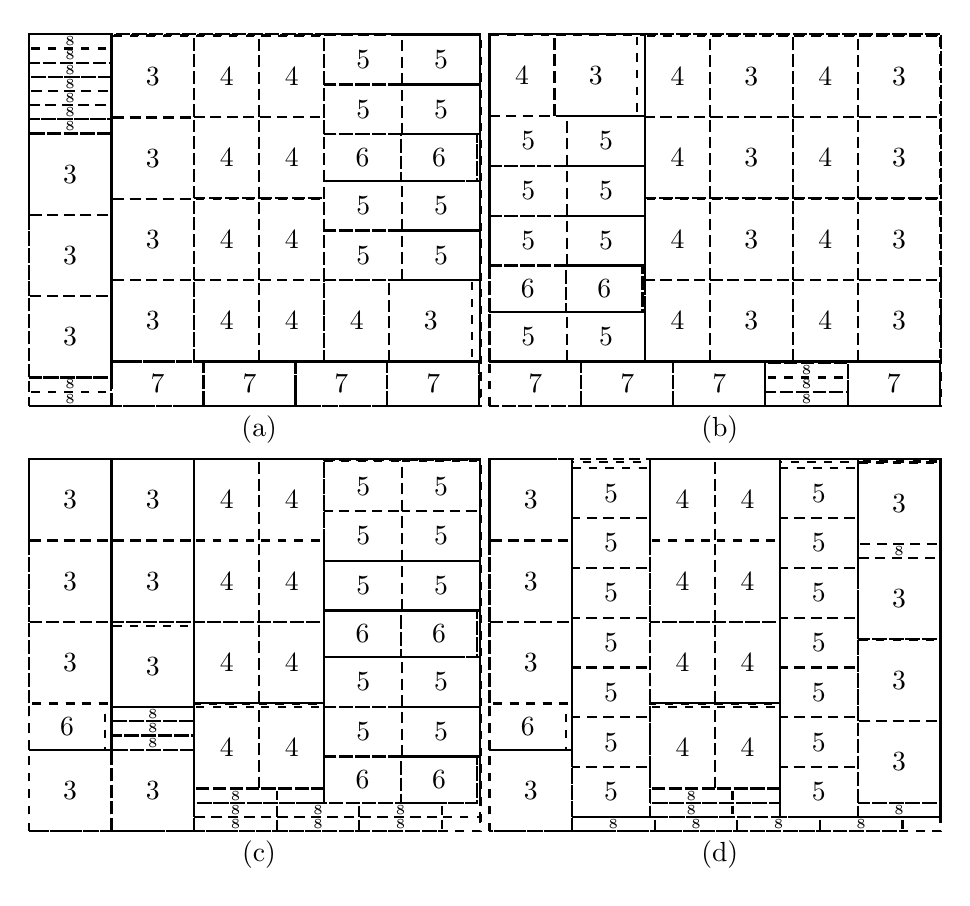
\begin{tikzpicture}[scale=0.225]
\def\labelfontsize{\normalsize}
\def\labelfontsizeeight{\tiny}
\def\firstpattern {
\draw[dashed, thick, black] (0.0, 0.0) rectangle (4.66, 0.8);
\node[font=\labelfontsizeeight] at (2.33, 0.4) {8};
%\node[font=\labelfontsize] at (2.33, 0.4) {466x80};
\draw[dashed, thick, black] (0.0, 0.8) rectangle (4.66, 1.6);
\node[font=\labelfontsizeeight] at (2.33, 1.2) {8};
%\node[font=\labelfontsize] at (2.33, 1.2) {466x80};
\draw[dashed, thick, black] (0.0, 0.0) rectangle (4.66, 1.6);
\draw[dashed, thick, black] (0.0, 1.6) rectangle (4.67, 6.19);
\node[font=\labelfontsize] at (2.335, 3.895) {3};
%\node[font=\labelfontsize] at (2.335, 3.895) {467x459};
\draw[dashed, thick, black] (0.0, 6.19) rectangle (4.67, 10.78);
\node[font=\labelfontsize] at (2.335, 8.485) {3};
%\node[font=\labelfontsize] at (2.335, 8.485) {467x459};
\draw[dashed, thick, black] (0.0, 10.78) rectangle (4.67, 15.37);
\node[font=\labelfontsize] at (2.335, 13.075) {3};
%\node[font=\labelfontsize] at (2.335, 13.075) {467x459};
\draw[dashed, thick, black] (0.0, 15.37) rectangle (4.66, 16.17);
\node[font=\labelfontsizeeight] at (2.33, 15.77) {8};
%\node[font=\labelfontsize] at (2.33, 15.77) {466x80};
\draw[dashed, thick, black] (0.0, 16.17) rectangle (4.66, 16.97);
\node[font=\labelfontsizeeight] at (2.33, 16.57) {8};
%\node[font=\labelfontsize] at (2.33, 16.57) {466x80};
\draw[dashed, thick, black] (0.0, 16.97) rectangle (4.66, 17.77);
\node[font=\labelfontsizeeight] at (2.33, 17.37) {8};
%\node[font=\labelfontsize] at (2.33, 17.37) {466x80};
\draw[dashed, thick, black] (0.0, 17.77) rectangle (4.66, 18.57);
\node[font=\labelfontsizeeight] at (2.33, 18.17) {8};
%\node[font=\labelfontsize] at (2.33, 18.17) {466x80};
\draw[dashed, thick, black] (0.0, 18.57) rectangle (4.66, 19.37);
\node[font=\labelfontsizeeight] at (2.33, 18.97) {8};
%\node[font=\labelfontsize] at (2.33, 18.97) {466x80};
\draw[dashed, thick, black] (0.0, 19.37) rectangle (4.66, 20.17);
\node[font=\labelfontsizeeight] at (2.33, 19.77) {8};
%\node[font=\labelfontsize] at (2.33, 19.77) {466x80};
\draw[dashed, thick, black] (0.0, 20.17) rectangle (4.66, 20.97);
\node[font=\labelfontsizeeight] at (2.33, 20.57) {8};
%\node[font=\labelfontsize] at (2.33, 20.57) {466x80};
\draw[dashed, thick, black] (0.0, 19.37) rectangle (4.66, 20.97);
\draw[dashed, thick, black] (0.0, 18.57) rectangle (4.66, 20.97);
\draw[dashed, thick, black] (0.0, 17.77) rectangle (4.66, 20.97);
\draw[dashed, thick, black] (0.0, 16.97) rectangle (4.66, 20.97);
\draw[dashed, thick, black] (0.0, 16.17) rectangle (4.67, 20.97);
\draw[dashed, thick, black] (0.0, 15.37) rectangle (4.67, 20.99);
\draw[dashed, thick, black] (0.0, 10.78) rectangle (4.67, 21.0);
\draw[dashed, thick, black] (0.0, 6.19) rectangle (4.67, 21.0);
\draw[dashed, thick, black] (0.0, 1.6) rectangle (4.67, 21.0);
\draw[dashed, thick, black] (0.0, 0.0) rectangle (4.67, 21.0);
\draw[dashed, thick, black] (4.67, 0.0) rectangle (9.86, 2.5);
\node[font=\labelfontsize] at (7.265, 1.25) {7};
%\node[font=\labelfontsize] at (7.265, 1.25) {519x250};
\draw[dashed, thick, black] (9.86, 0.0) rectangle (15.05, 2.5);
\node[font=\labelfontsize] at (12.455, 1.25) {7};
%\node[font=\labelfontsize] at (12.455, 1.25) {519x250};
\draw[dashed, thick, black] (4.67, 0.0) rectangle (15.05, 2.5);
\draw[dashed, thick, black] (15.05, 0.0) rectangle (20.24, 2.5);
\node[font=\labelfontsize] at (17.645, 1.25) {7};
%\node[font=\labelfontsize] at (17.645, 1.25) {519x250};
\draw[dashed, thick, black] (20.24, 0.0) rectangle (25.43, 2.5);
\node[font=\labelfontsize] at (22.835, 1.25) {7};
%\node[font=\labelfontsize] at (22.835, 1.25) {519x250};
\draw[dashed, thick, black] (15.05, 0.0) rectangle (25.43, 2.5);
\draw[dashed, thick, black] (4.67, 0.0) rectangle (25.43, 2.5);
\draw[dashed, thick, black] (4.67, 2.5) rectangle (9.34, 7.09);
\node[font=\labelfontsize] at (7.005, 4.795) {3};
%\node[font=\labelfontsize] at (7.005, 4.795) {467x459};
\draw[dashed, thick, black] (4.67, 7.09) rectangle (9.34, 11.68);
\node[font=\labelfontsize] at (7.005, 9.385) {3};
%\node[font=\labelfontsize] at (7.005, 9.385) {467x459};
\draw[dashed, thick, black] (4.67, 2.5) rectangle (9.34, 11.68);
\draw[dashed, thick, black] (4.67, 11.68) rectangle (9.34, 16.27);
\node[font=\labelfontsize] at (7.005, 13.975) {3};
%\node[font=\labelfontsize] at (7.005, 13.975) {467x459};
\draw[dashed, thick, black] (4.67, 16.27) rectangle (9.34, 20.86);
\node[font=\labelfontsize] at (7.005, 18.565) {3};
%\node[font=\labelfontsize] at (7.005, 18.565) {467x459};
\draw[dashed, thick, black] (4.67, 11.68) rectangle (9.34, 20.91);
\draw[dashed, thick, black] (4.67, 2.5) rectangle (9.34, 20.97);
\draw[dashed, thick, black] (9.34, 2.5) rectangle (13.01, 7.09);
\node[font=\labelfontsize] at (11.175, 4.795) {4};
%\node[font=\labelfontsize] at (11.175, 4.795) {367x459};
\draw[dashed, thick, black] (13.01, 2.5) rectangle (16.68, 7.09);
\node[font=\labelfontsize] at (14.845, 4.795) {4};
%\node[font=\labelfontsize] at (14.845, 4.795) {367x459};
\draw[dashed, thick, black] (9.34, 2.5) rectangle (16.68, 7.09);
\draw[dashed, thick, black] (9.34, 7.09) rectangle (13.01, 11.68);
\node[font=\labelfontsize] at (11.175, 9.385) {4};
%\node[font=\labelfontsize] at (11.175, 9.385) {367x459};
\draw[dashed, thick, black] (13.01, 7.09) rectangle (16.68, 11.68);
\node[font=\labelfontsize] at (14.845, 9.385) {4};
%\node[font=\labelfontsize] at (14.845, 9.385) {367x459};
\draw[dashed, thick, black] (9.34, 7.09) rectangle (16.68, 11.68);
\draw[dashed, thick, black] (9.34, 2.5) rectangle (16.68, 11.71);
\draw[dashed, thick, black] (9.34, 11.71) rectangle (13.01, 16.3);
\node[font=\labelfontsize] at (11.175, 14.005) {4};
%\node[font=\labelfontsize] at (11.175, 14.005) {367x459};
\draw[dashed, thick, black] (13.01, 11.71) rectangle (16.68, 16.3);
\node[font=\labelfontsize] at (14.845, 14.005) {4};
%\node[font=\labelfontsize] at (14.845, 14.005) {367x459};
\draw[dashed, thick, black] (9.34, 11.71) rectangle (16.68, 16.3);
\draw[dashed, thick, black] (9.34, 16.3) rectangle (13.01, 20.89);
\node[font=\labelfontsize] at (11.175, 18.595) {4};
%\node[font=\labelfontsize] at (11.175, 18.595) {367x459};
\draw[dashed, thick, black] (13.01, 16.3) rectangle (16.68, 20.89);
\node[font=\labelfontsize] at (14.845, 18.595) {4};
%\node[font=\labelfontsize] at (14.845, 18.595) {367x459};
\draw[dashed, thick, black] (9.34, 16.3) rectangle (16.68, 20.89);
\draw[dashed, thick, black] (9.34, 11.71) rectangle (16.68, 20.94);
\draw[dashed, thick, black] (9.34, 2.5) rectangle (16.68, 21.0);
\draw[dashed, thick, black] (16.68, 2.5) rectangle (20.35, 7.09);
\node[font=\labelfontsize] at (18.515, 4.795) {4};
%\node[font=\labelfontsize] at (18.515, 4.795) {367x459};
\draw[dashed, thick, black] (20.35, 2.5) rectangle (25.02, 7.09);
\node[font=\labelfontsize] at (22.685, 4.795) {3};
%\node[font=\labelfontsize] at (22.685, 4.795) {467x459};
\draw[dashed, thick, black] (16.68, 2.5) rectangle (25.46, 7.09);
\draw[dashed, thick, black] (16.68, 7.09) rectangle (21.07, 9.9);
\node[font=\labelfontsize] at (18.875, 8.495) {5};
%\node[font=\labelfontsize] at (18.875, 8.495) {439x281};
\draw[dashed, thick, black] (21.07, 7.09) rectangle (25.46, 9.9);
\node[font=\labelfontsize] at (23.265, 8.495) {5};
%\node[font=\labelfontsize] at (23.265, 8.495) {439x281};
\draw[dashed, thick, black] (16.68, 7.09) rectangle (25.46, 9.9);
\draw[dashed, thick, black] (16.68, 9.9) rectangle (21.07, 12.71);
\node[font=\labelfontsize] at (18.875, 11.305) {5};
%\node[font=\labelfontsize] at (18.875, 11.305) {439x281};
\draw[dashed, thick, black] (21.07, 9.9) rectangle (25.46, 12.71);
\node[font=\labelfontsize] at (23.265, 11.305) {5};
%\node[font=\labelfontsize] at (23.265, 11.305) {439x281};
\draw[dashed, thick, black] (16.68, 9.9) rectangle (25.46, 12.71);
\draw[dashed, thick, black] (16.68, 7.09) rectangle (25.46, 12.71);
\draw[dashed, thick, black] (16.68, 12.71) rectangle (21.0, 15.32);
\node[font=\labelfontsize] at (18.84, 14.015) {6};
%\node[font=\labelfontsize] at (18.84, 14.015) {432x261};
\draw[dashed, thick, black] (21.0, 12.71) rectangle (25.32, 15.32);
\node[font=\labelfontsize] at (23.16, 14.015) {6};
%\node[font=\labelfontsize] at (23.16, 14.015) {432x261};
\draw[dashed, thick, black] (16.68, 12.71) rectangle (25.32, 15.32);
\draw[dashed, thick, black] (16.68, 15.32) rectangle (21.07, 18.13);
\node[font=\labelfontsize] at (18.875, 16.725) {5};
%\node[font=\labelfontsize] at (18.875, 16.725) {439x281};
\draw[dashed, thick, black] (21.07, 15.32) rectangle (25.46, 18.13);
\node[font=\labelfontsize] at (23.265, 16.725) {5};
%\node[font=\labelfontsize] at (23.265, 16.725) {439x281};
\draw[dashed, thick, black] (16.68, 15.32) rectangle (25.46, 18.13);
\draw[dashed, thick, black] (16.68, 18.13) rectangle (21.07, 20.94);
\node[font=\labelfontsize] at (18.875, 19.535) {5};
%\node[font=\labelfontsize] at (18.875, 19.535) {439x281};
\draw[dashed, thick, black] (21.07, 18.13) rectangle (25.46, 20.94);
\node[font=\labelfontsize] at (23.265, 19.535) {5};
%\node[font=\labelfontsize] at (23.265, 19.535) {439x281};
\draw[dashed, thick, black] (16.68, 18.13) rectangle (25.46, 20.94);
\draw[dashed, thick, black] (16.68, 15.32) rectangle (25.46, 20.94);
\draw[dashed, thick, black] (16.68, 12.71) rectangle (25.46, 20.94);
\draw[dashed, thick, black] (16.68, 7.09) rectangle (25.46, 21.0);
\draw[dashed, thick, black] (16.68, 2.5) rectangle (25.46, 21.0);
\draw[dashed, thick, black] (9.34, 2.5) rectangle (25.46, 21.0);
\draw[dashed, thick, black] (4.67, 2.5) rectangle (25.46, 21.0);
\draw[dashed, thick, black] (4.67, 0.0) rectangle (25.46, 21.0);
\draw[dashed, thick, black] (0.0, 0.0) rectangle (25.5, 21.0);
}
\def\secondpattern {
\draw[dashed, thick, black] (0.0, 0.0) rectangle (5.19, 2.5);
\node[font=\labelfontsize] at (2.595, 1.25) {7};
%\node[font=\labelfontsize] at (2.595, 1.25) {519x250};
\draw[dashed, thick, black] (5.19, 0.0) rectangle (10.38, 2.5);
\node[font=\labelfontsize] at (7.785, 1.25) {7};
%\node[font=\labelfontsize] at (7.785, 1.25) {519x250};
\draw[dashed, thick, black] (10.38, 0.0) rectangle (15.57, 2.5);
\node[font=\labelfontsize] at (12.975, 1.25) {7};
%\node[font=\labelfontsize] at (12.975, 1.25) {519x250};
\draw[dashed, thick, black] (15.57, 0.0) rectangle (20.23, 0.8);
\node[font=\labelfontsizeeight] at (17.9, 0.4) {8};
%\node[font=\labelfontsize] at (17.9, 0.4) {466x80};
\draw[dashed, thick, black] (15.57, 0.8) rectangle (20.23, 1.6);
\node[font=\labelfontsizeeight] at (17.9, 1.2) {8};
%\node[font=\labelfontsize] at (17.9, 1.2) {466x80};
\draw[dashed, thick, black] (15.57, 1.6) rectangle (20.23, 2.4);
\node[font=\labelfontsizeeight] at (17.9, 2.0) {8};
%\node[font=\labelfontsize] at (17.9, 2.0) {466x80};
\draw[dashed, thick, black] (15.57, 0.8) rectangle (20.23, 2.4);
\draw[dashed, thick, black] (15.57, 0.0) rectangle (20.23, 2.4);
\draw[dashed, thick, black] (20.23, 0.0) rectangle (25.42, 2.5);
\node[font=\labelfontsize] at (22.825, 1.25) {7};
%\node[font=\labelfontsize] at (22.825, 1.25) {519x250};
\draw[dashed, thick, black] (15.57, 0.0) rectangle (25.42, 2.5);
\draw[dashed, thick, black] (10.38, 0.0) rectangle (25.42, 2.5);
\draw[dashed, thick, black] (5.19, 0.0) rectangle (25.42, 2.5);
\draw[dashed, thick, black] (0.0, 0.0) rectangle (25.42, 2.5);
\draw[dashed, thick, black] (0.0, 2.5) rectangle (4.39, 5.31);
\node[font=\labelfontsize] at (2.195, 3.905) {5};
%\node[font=\labelfontsize] at (2.195, 3.905) {439x281};
\draw[dashed, thick, black] (4.39, 2.5) rectangle (8.78, 5.31);
\node[font=\labelfontsize] at (6.585, 3.905) {5};
%\node[font=\labelfontsize] at (6.585, 3.905) {439x281};
\draw[dashed, thick, black] (0.0, 2.5) rectangle (8.78, 5.31);
\draw[dashed, thick, black] (0.0, 5.31) rectangle (4.32, 7.92);
\node[font=\labelfontsize] at (2.16, 6.615) {6};
%\node[font=\labelfontsize] at (2.16, 6.615) {432x261};
\draw[dashed, thick, black] (4.32, 5.31) rectangle (8.64, 7.92);
\node[font=\labelfontsize] at (6.48, 6.615) {6};
%\node[font=\labelfontsize] at (6.48, 6.615) {432x261};
\draw[dashed, thick, black] (0.0, 5.31) rectangle (8.64, 7.92);
\draw[dashed, thick, black] (0.0, 7.92) rectangle (4.39, 10.73);
\node[font=\labelfontsize] at (2.195, 9.325) {5};
%\node[font=\labelfontsize] at (2.195, 9.325) {439x281};
\draw[dashed, thick, black] (4.39, 7.92) rectangle (8.78, 10.73);
\node[font=\labelfontsize] at (6.585, 9.325) {5};
%\node[font=\labelfontsize] at (6.585, 9.325) {439x281};
\draw[dashed, thick, black] (0.0, 7.92) rectangle (8.78, 10.73);
\draw[dashed, thick, black] (0.0, 5.31) rectangle (8.78, 10.73);
\draw[dashed, thick, black] (0.0, 2.5) rectangle (8.78, 10.73);
\draw[dashed, thick, black] (0.0, 10.73) rectangle (4.39, 13.54);
\node[font=\labelfontsize] at (2.195, 12.135) {5};
%\node[font=\labelfontsize] at (2.195, 12.135) {439x281};
\draw[dashed, thick, black] (4.39, 10.73) rectangle (8.78, 13.54);
\node[font=\labelfontsize] at (6.585, 12.135) {5};
%\node[font=\labelfontsize] at (6.585, 12.135) {439x281};
\draw[dashed, thick, black] (0.0, 10.73) rectangle (8.78, 13.54);
\draw[dashed, thick, black] (0.0, 13.54) rectangle (4.39, 16.35);
\node[font=\labelfontsize] at (2.195, 14.945) {5};
%\node[font=\labelfontsize] at (2.195, 14.945) {439x281};
\draw[dashed, thick, black] (4.39, 13.54) rectangle (8.78, 16.35);
\node[font=\labelfontsize] at (6.585, 14.945) {5};
%\node[font=\labelfontsize] at (6.585, 14.945) {439x281};
\draw[dashed, thick, black] (0.0, 13.54) rectangle (8.78, 16.35);
\draw[dashed, thick, black] (0.0, 16.35) rectangle (3.67, 20.94);
\node[font=\labelfontsize] at (1.835, 18.645) {4};
%\node[font=\labelfontsize] at (1.835, 18.645) {367x459};
\draw[dashed, thick, black] (3.67, 16.35) rectangle (8.34, 20.94);
\node[font=\labelfontsize] at (6.005, 18.645) {3};
%\node[font=\labelfontsize] at (6.005, 18.645) {467x459};
\draw[dashed, thick, black] (0.0, 16.35) rectangle (8.78, 20.94);
\draw[dashed, thick, black] (0.0, 13.54) rectangle (8.78, 20.95);
\draw[dashed, thick, black] (0.0, 10.73) rectangle (8.78, 20.96);
\draw[dashed, thick, black] (0.0, 2.5) rectangle (8.78, 21.0);
\draw[dashed, thick, black] (8.78, 2.5) rectangle (12.45, 7.09);
\node[font=\labelfontsize] at (10.615, 4.795) {4};
%\node[font=\labelfontsize] at (10.615, 4.795) {367x459};
\draw[dashed, thick, black] (12.45, 2.5) rectangle (17.12, 7.09);
\node[font=\labelfontsize] at (14.785, 4.795) {3};
%\node[font=\labelfontsize] at (14.785, 4.795) {467x459};
\draw[dashed, thick, black] (8.78, 2.5) rectangle (17.12, 7.09);
\draw[dashed, thick, black] (17.12, 2.5) rectangle (20.79, 7.09);
\node[font=\labelfontsize] at (18.955, 4.795) {4};
%\node[font=\labelfontsize] at (18.955, 4.795) {367x459};
\draw[dashed, thick, black] (20.79, 2.5) rectangle (25.46, 7.09);
\node[font=\labelfontsize] at (23.125, 4.795) {3};
%\node[font=\labelfontsize] at (23.125, 4.795) {467x459};
\draw[dashed, thick, black] (17.12, 2.5) rectangle (25.46, 7.09);
\draw[dashed, thick, black] (8.78, 2.5) rectangle (25.48, 7.09);
\draw[dashed, thick, black] (8.78, 7.09) rectangle (12.45, 11.68);
\node[font=\labelfontsize] at (10.615, 9.385) {4};
%\node[font=\labelfontsize] at (10.615, 9.385) {367x459};
\draw[dashed, thick, black] (12.45, 7.09) rectangle (17.12, 11.68);
\node[font=\labelfontsize] at (14.785, 9.385) {3};
%\node[font=\labelfontsize] at (14.785, 9.385) {467x459};
\draw[dashed, thick, black] (8.78, 7.09) rectangle (17.12, 11.68);
\draw[dashed, thick, black] (17.12, 7.09) rectangle (20.79, 11.68);
\node[font=\labelfontsize] at (18.955, 9.385) {4};
%\node[font=\labelfontsize] at (18.955, 9.385) {367x459};
\draw[dashed, thick, black] (20.79, 7.09) rectangle (25.46, 11.68);
\node[font=\labelfontsize] at (23.125, 9.385) {3};
%\node[font=\labelfontsize] at (23.125, 9.385) {467x459};
\draw[dashed, thick, black] (17.12, 7.09) rectangle (25.46, 11.68);
\draw[dashed, thick, black] (8.78, 7.09) rectangle (25.48, 11.68);
\draw[dashed, thick, black] (8.78, 2.5) rectangle (25.48, 11.72);
\draw[dashed, thick, black] (8.78, 11.72) rectangle (12.45, 16.31);
\node[font=\labelfontsize] at (10.615, 14.015) {4};
%\node[font=\labelfontsize] at (10.615, 14.015) {367x459};
\draw[dashed, thick, black] (12.45, 11.72) rectangle (17.12, 16.31);
\node[font=\labelfontsize] at (14.785, 14.015) {3};
%\node[font=\labelfontsize] at (14.785, 14.015) {467x459};
\draw[dashed, thick, black] (8.78, 11.72) rectangle (17.12, 16.31);
\draw[dashed, thick, black] (17.12, 11.72) rectangle (20.79, 16.31);
\node[font=\labelfontsize] at (18.955, 14.015) {4};
%\node[font=\labelfontsize] at (18.955, 14.015) {367x459};
\draw[dashed, thick, black] (20.79, 11.72) rectangle (25.46, 16.31);
\node[font=\labelfontsize] at (23.125, 14.015) {3};
%\node[font=\labelfontsize] at (23.125, 14.015) {467x459};
\draw[dashed, thick, black] (17.12, 11.72) rectangle (25.46, 16.31);
\draw[dashed, thick, black] (8.78, 11.72) rectangle (25.48, 16.31);
\draw[dashed, thick, black] (8.78, 16.31) rectangle (12.45, 20.9);
\node[font=\labelfontsize] at (10.615, 18.605) {4};
%\node[font=\labelfontsize] at (10.615, 18.605) {367x459};
\draw[dashed, thick, black] (12.45, 16.31) rectangle (17.12, 20.9);
\node[font=\labelfontsize] at (14.785, 18.605) {3};
%\node[font=\labelfontsize] at (14.785, 18.605) {467x459};
\draw[dashed, thick, black] (8.78, 16.31) rectangle (17.12, 20.9);
\draw[dashed, thick, black] (17.12, 16.31) rectangle (20.79, 20.9);
\node[font=\labelfontsize] at (18.955, 18.605) {4};
%\node[font=\labelfontsize] at (18.955, 18.605) {367x459};
\draw[dashed, thick, black] (20.79, 16.31) rectangle (25.46, 20.9);
\node[font=\labelfontsize] at (23.125, 18.605) {3};
%\node[font=\labelfontsize] at (23.125, 18.605) {467x459};
\draw[dashed, thick, black] (17.12, 16.31) rectangle (25.46, 20.9);
\draw[dashed, thick, black] (8.78, 16.31) rectangle (25.48, 20.9);
\draw[dashed, thick, black] (8.78, 11.72) rectangle (25.48, 20.95);
\draw[dashed, thick, black] (8.78, 2.5) rectangle (25.48, 21.0);
\draw[dashed, thick, black] (0.0, 2.5) rectangle (25.49, 21.0);
\draw[dashed, thick, black] (0.0, 0.0) rectangle (25.5, 21.0);
}
\def\thirdpattern {
\draw[dashed, thick, black] (0.0, 0.0) rectangle (4.67, 4.59);
\node[font=\labelfontsize] at (2.335, 2.295) {3};
%\node[font=\labelfontsize] at (2.335, 2.295) {467x459};
\draw[dashed, thick, black] (0.0, 4.59) rectangle (4.32, 7.2);
\node[font=\labelfontsize] at (2.16, 5.895) {6};
%\node[font=\labelfontsize] at (2.16, 5.895) {432x261};
\draw[dashed, thick, black] (0.0, 4.59) rectangle (4.66, 7.2);
\draw[dashed, thick, black] (0.0, 7.2) rectangle (4.67, 11.79);
\node[font=\labelfontsize] at (2.335, 9.495) {3};
%\node[font=\labelfontsize] at (2.335, 9.495) {467x459};
\draw[dashed, thick, black] (0.0, 4.59) rectangle (4.67, 11.81);
\draw[dashed, thick, black] (0.0, 11.81) rectangle (4.67, 16.4);
\node[font=\labelfontsize] at (2.335, 14.105) {3};
%\node[font=\labelfontsize] at (2.335, 14.105) {467x459};
\draw[dashed, thick, black] (0.0, 16.4) rectangle (4.67, 20.99);
\node[font=\labelfontsize] at (2.335, 18.695) {3};
%\node[font=\labelfontsize] at (2.335, 18.695) {467x459};
\draw[dashed, thick, black] (0.0, 11.81) rectangle (4.67, 20.99);
\draw[dashed, thick, black] (0.0, 4.59) rectangle (4.67, 21.0);
\draw[dashed, thick, black] (0.0, 0.0) rectangle (4.67, 21.0);
\draw[dashed, thick, black] (4.67, 0.0) rectangle (9.34, 4.59);
\node[font=\labelfontsize] at (7.005, 2.295) {3};
%\node[font=\labelfontsize] at (7.005, 2.295) {467x459};
\draw[dashed, thick, black] (4.67, 4.59) rectangle (9.33, 5.39);
\node[font=\labelfontsizeeight] at (7.0, 4.99) {8};
%\node[font=\labelfontsize] at (7.0, 4.99) {466x80};
\draw[dashed, thick, black] (4.67, 5.39) rectangle (9.33, 6.19);
\node[font=\labelfontsizeeight] at (7.0, 5.79) {8};
%\node[font=\labelfontsize] at (7.0, 5.79) {466x80};
\draw[dashed, thick, black] (4.67, 6.19) rectangle (9.33, 6.99);
\node[font=\labelfontsizeeight] at (7.0, 6.59) {8};
%\node[font=\labelfontsize] at (7.0, 6.59) {466x80};
\draw[dashed, thick, black] (4.67, 6.99) rectangle (9.34, 11.58);
\node[font=\labelfontsize] at (7.005, 9.285) {3};
%\node[font=\labelfontsize] at (7.005, 9.285) {467x459};
\draw[dashed, thick, black] (4.67, 6.99) rectangle (9.34, 11.79);
\draw[dashed, thick, black] (4.67, 6.19) rectangle (9.34, 11.81);
\draw[dashed, thick, black] (4.67, 11.81) rectangle (9.34, 16.4);
\node[font=\labelfontsize] at (7.005, 14.105) {3};
%\node[font=\labelfontsize] at (7.005, 14.105) {467x459};
\draw[dashed, thick, black] (4.67, 16.4) rectangle (9.34, 20.99);
\node[font=\labelfontsize] at (7.005, 18.695) {3};
%\node[font=\labelfontsize] at (7.005, 18.695) {467x459};
\draw[dashed, thick, black] (4.67, 11.81) rectangle (9.34, 20.99);
\draw[dashed, thick, black] (4.67, 6.19) rectangle (9.34, 21.0);
\draw[dashed, thick, black] (4.67, 5.39) rectangle (9.34, 21.0);
\draw[dashed, thick, black] (4.67, 4.59) rectangle (9.34, 21.0);
\draw[dashed, thick, black] (4.67, 0.0) rectangle (9.34, 21.0);
\draw[dashed, thick, black] (9.34, 0.0) rectangle (14.0, 0.8);
\node[font=\labelfontsizeeight] at (11.67, 0.4) {8};
%\node[font=\labelfontsize] at (11.67, 0.4) {466x80};
\draw[dashed, thick, black] (14.0, 0.0) rectangle (18.66, 0.8);
\node[font=\labelfontsizeeight] at (16.33, 0.4) {8};
%\node[font=\labelfontsize] at (16.33, 0.4) {466x80};
\draw[dashed, thick, black] (18.66, 0.0) rectangle (23.32, 0.8);
\node[font=\labelfontsizeeight] at (20.99, 0.4) {8};
%\node[font=\labelfontsize] at (20.99, 0.4) {466x80};
\draw[dashed, thick, black] (14.0, 0.0) rectangle (23.32, 0.8);
\draw[dashed, thick, black] (9.34, 0.0) rectangle (23.32, 0.8);
\draw[dashed, thick, black] (9.34, 0.8) rectangle (14.0, 1.6);
\node[font=\labelfontsizeeight] at (11.67, 1.2) {8};
%\node[font=\labelfontsize] at (11.67, 1.2) {466x80};
\draw[dashed, thick, black] (14.0, 0.8) rectangle (18.66, 1.6);
\node[font=\labelfontsizeeight] at (16.33, 1.2) {8};
%\node[font=\labelfontsize] at (16.33, 1.2) {466x80};
\draw[dashed, thick, black] (18.66, 0.8) rectangle (23.32, 1.6);
\node[font=\labelfontsizeeight] at (20.99, 1.2) {8};
%\node[font=\labelfontsize] at (20.99, 1.2) {466x80};
\draw[dashed, thick, black] (14.0, 0.8) rectangle (23.32, 1.6);
\draw[dashed, thick, black] (9.34, 0.8) rectangle (23.32, 1.6);
\draw[dashed, thick, black] (9.34, 1.6) rectangle (14.0, 2.4);
\node[font=\labelfontsizeeight] at (11.67, 2.0) {8};
%\node[font=\labelfontsize] at (11.67, 2.0) {466x80};
\draw[dashed, thick, black] (9.34, 2.4) rectangle (13.01, 6.99);
\node[font=\labelfontsize] at (11.175, 4.695) {4};
%\node[font=\labelfontsize] at (11.175, 4.695) {367x459};
\draw[dashed, thick, black] (13.01, 2.4) rectangle (16.68, 6.99);
\node[font=\labelfontsize] at (14.845, 4.695) {4};
%\node[font=\labelfontsize] at (14.845, 4.695) {367x459};
\draw[dashed, thick, black] (9.34, 2.4) rectangle (16.68, 7.2);
\draw[dashed, thick, black] (9.34, 1.6) rectangle (16.68, 7.22);
\draw[dashed, thick, black] (9.34, 7.22) rectangle (13.01, 11.81);
\node[font=\labelfontsize] at (11.175, 9.515) {4};
%\node[font=\labelfontsize] at (11.175, 9.515) {367x459};
\draw[dashed, thick, black] (13.01, 7.22) rectangle (16.68, 11.81);
\node[font=\labelfontsize] at (14.845, 9.515) {4};
%\node[font=\labelfontsize] at (14.845, 9.515) {367x459};
\draw[dashed, thick, black] (9.34, 7.22) rectangle (16.68, 11.81);
\draw[dashed, thick, black] (9.34, 11.81) rectangle (13.01, 16.4);
\node[font=\labelfontsize] at (11.175, 14.105) {4};
%\node[font=\labelfontsize] at (11.175, 14.105) {367x459};
\draw[dashed, thick, black] (9.34, 16.4) rectangle (13.01, 20.99);
\node[font=\labelfontsize] at (11.175, 18.695) {4};
%\node[font=\labelfontsize] at (11.175, 18.695) {367x459};
\draw[dashed, thick, black] (9.34, 11.81) rectangle (13.01, 20.99);
\draw[dashed, thick, black] (13.01, 11.81) rectangle (16.68, 16.4);
\node[font=\labelfontsize] at (14.845, 14.105) {4};
%\node[font=\labelfontsize] at (14.845, 14.105) {367x459};
\draw[dashed, thick, black] (13.01, 16.4) rectangle (16.68, 20.99);
\node[font=\labelfontsize] at (14.845, 18.695) {4};
%\node[font=\labelfontsize] at (14.845, 18.695) {367x459};
\draw[dashed, thick, black] (13.01, 11.81) rectangle (16.68, 20.99);
\draw[dashed, thick, black] (9.34, 11.81) rectangle (16.68, 20.99);
\draw[dashed, thick, black] (9.34, 7.22) rectangle (16.68, 20.99);
\draw[dashed, thick, black] (9.34, 1.6) rectangle (16.68, 21.0);
\draw[dashed, thick, black] (16.68, 1.6) rectangle (21.0, 4.21);
\node[font=\labelfontsize] at (18.84, 2.905) {6};
%\node[font=\labelfontsize] at (18.84, 2.905) {432x261};
\draw[dashed, thick, black] (21.0, 1.6) rectangle (25.32, 4.21);
\node[font=\labelfontsize] at (23.16, 2.905) {6};
%\node[font=\labelfontsize] at (23.16, 2.905) {432x261};
\draw[dashed, thick, black] (16.68, 1.6) rectangle (25.32, 4.21);
\draw[dashed, thick, black] (16.68, 4.21) rectangle (21.07, 7.02);
\node[font=\labelfontsize] at (18.875, 5.615) {5};
%\node[font=\labelfontsize] at (18.875, 5.615) {439x281};
\draw[dashed, thick, black] (21.07, 4.21) rectangle (25.46, 7.02);
\node[font=\labelfontsize] at (23.265, 5.615) {5};
%\node[font=\labelfontsize] at (23.265, 5.615) {439x281};
\draw[dashed, thick, black] (16.68, 4.21) rectangle (25.46, 7.02);
\draw[dashed, thick, black] (16.68, 7.02) rectangle (21.07, 9.83);
\node[font=\labelfontsize] at (18.875, 8.425) {5};
%\node[font=\labelfontsize] at (18.875, 8.425) {439x281};
\draw[dashed, thick, black] (21.07, 7.02) rectangle (25.46, 9.83);
\node[font=\labelfontsize] at (23.265, 8.425) {5};
%\node[font=\labelfontsize] at (23.265, 8.425) {439x281};
\draw[dashed, thick, black] (16.68, 7.02) rectangle (25.46, 9.83);
\draw[dashed, thick, black] (16.68, 4.21) rectangle (25.46, 9.83);
\draw[dashed, thick, black] (16.68, 9.83) rectangle (21.0, 12.44);
\node[font=\labelfontsize] at (18.84, 11.135) {6};
%\node[font=\labelfontsize] at (18.84, 11.135) {432x261};
\draw[dashed, thick, black] (21.0, 9.83) rectangle (25.32, 12.44);
\node[font=\labelfontsize] at (23.16, 11.135) {6};
%\node[font=\labelfontsize] at (23.16, 11.135) {432x261};
\draw[dashed, thick, black] (16.68, 9.83) rectangle (25.32, 12.44);
\draw[dashed, thick, black] (16.68, 12.44) rectangle (21.07, 15.25);
\node[font=\labelfontsize] at (18.875, 13.845) {5};
%\node[font=\labelfontsize] at (18.875, 13.845) {439x281};
\draw[dashed, thick, black] (21.07, 12.44) rectangle (25.46, 15.25);
\node[font=\labelfontsize] at (23.265, 13.845) {5};
%\node[font=\labelfontsize] at (23.265, 13.845) {439x281};
\draw[dashed, thick, black] (16.68, 12.44) rectangle (25.46, 15.25);
\draw[dashed, thick, black] (16.68, 15.25) rectangle (21.07, 18.06);
\node[font=\labelfontsize] at (18.875, 16.655) {5};
%\node[font=\labelfontsize] at (18.875, 16.655) {439x281};
\draw[dashed, thick, black] (16.68, 18.06) rectangle (21.07, 20.87);
\node[font=\labelfontsize] at (18.875, 19.465) {5};
%\node[font=\labelfontsize] at (18.875, 19.465) {439x281};
\draw[dashed, thick, black] (16.68, 15.25) rectangle (21.07, 20.87);
\draw[dashed, thick, black] (21.07, 15.25) rectangle (25.46, 18.06);
\node[font=\labelfontsize] at (23.265, 16.655) {5};
%\node[font=\labelfontsize] at (23.265, 16.655) {439x281};
\draw[dashed, thick, black] (21.07, 18.06) rectangle (25.46, 20.87);
\node[font=\labelfontsize] at (23.265, 19.465) {5};
%\node[font=\labelfontsize] at (23.265, 19.465) {439x281};
\draw[dashed, thick, black] (21.07, 15.25) rectangle (25.46, 20.87);
\draw[dashed, thick, black] (16.68, 15.25) rectangle (25.46, 20.95);
\draw[dashed, thick, black] (16.68, 12.44) rectangle (25.46, 20.96);
\draw[dashed, thick, black] (16.68, 9.83) rectangle (25.46, 20.96);
\draw[dashed, thick, black] (16.68, 4.21) rectangle (25.46, 21.0);
\draw[dashed, thick, black] (16.68, 1.6) rectangle (25.46, 21.0);
\draw[dashed, thick, black] (9.34, 1.6) rectangle (25.46, 21.0);
\draw[dashed, thick, black] (9.34, 0.8) rectangle (25.46, 21.0);
\draw[dashed, thick, black] (9.34, 0.0) rectangle (25.46, 21.0);
\draw[dashed, thick, black] (4.67, 0.0) rectangle (25.46, 21.0);
\draw[dashed, thick, black] (0.0, 0.0) rectangle (25.5, 21.0);
}
\def\fourthpattern {
\draw[dashed, thick, black] (0.0, 0.0) rectangle (4.67, 4.59);
\node[font=\labelfontsize] at (2.335, 2.295) {3};
%\node[font=\labelfontsize] at (2.335, 2.295) {467x459};
\draw[dashed, thick, black] (0.0, 4.59) rectangle (4.32, 7.2);
\node[font=\labelfontsize] at (2.16, 5.895) {6};
%\node[font=\labelfontsize] at (2.16, 5.895) {432x261};
\draw[dashed, thick, black] (0.0, 4.59) rectangle (4.66, 7.2);
\draw[dashed, thick, black] (0.0, 7.2) rectangle (4.67, 11.79);
\node[font=\labelfontsize] at (2.335, 9.495) {3};
%\node[font=\labelfontsize] at (2.335, 9.495) {467x459};
\draw[dashed, thick, black] (0.0, 4.59) rectangle (4.67, 11.81);
\draw[dashed, thick, black] (0.0, 11.81) rectangle (4.67, 16.4);
\node[font=\labelfontsize] at (2.335, 14.105) {3};
%\node[font=\labelfontsize] at (2.335, 14.105) {467x459};
\draw[dashed, thick, black] (0.0, 16.4) rectangle (4.67, 20.99);
\node[font=\labelfontsize] at (2.335, 18.695) {3};
%\node[font=\labelfontsize] at (2.335, 18.695) {467x459};
\draw[dashed, thick, black] (0.0, 11.81) rectangle (4.67, 20.99);
\draw[dashed, thick, black] (0.0, 4.59) rectangle (4.67, 21.0);
\draw[dashed, thick, black] (0.0, 0.0) rectangle (4.67, 21.0);
\draw[dashed, thick, black] (4.67, 0.0) rectangle (9.33, 0.8);
\node[font=\labelfontsizeeight] at (7.0, 0.4) {8};
%\node[font=\labelfontsize] at (7.0, 0.4) {466x80};
\draw[dashed, thick, black] (9.33, 0.0) rectangle (13.99, 0.8);
\node[font=\labelfontsizeeight] at (11.66, 0.4) {8};
%\node[font=\labelfontsize] at (11.66, 0.4) {466x80};
\draw[dashed, thick, black] (13.99, 0.0) rectangle (18.65, 0.8);
\node[font=\labelfontsizeeight] at (16.32, 0.4) {8};
%\node[font=\labelfontsize] at (16.32, 0.4) {466x80};
\draw[dashed, thick, black] (18.65, 0.0) rectangle (23.31, 0.8);
\node[font=\labelfontsizeeight] at (20.98, 0.4) {8};
%\node[font=\labelfontsize] at (20.98, 0.4) {466x80};
\draw[dashed, thick, black] (13.99, 0.0) rectangle (23.31, 0.8);
\draw[dashed, thick, black] (9.33, 0.0) rectangle (23.31, 0.8);
\draw[dashed, thick, black] (4.67, 0.0) rectangle (23.31, 0.8);
\draw[dashed, thick, black] (4.67, 0.8) rectangle (9.06, 3.61);
\node[font=\labelfontsize] at (6.865, 2.205) {5};
%\node[font=\labelfontsize] at (6.865, 2.205) {439x281};
\draw[dashed, thick, black] (4.67, 3.61) rectangle (9.06, 6.42);
\node[font=\labelfontsize] at (6.865, 5.015) {5};
%\node[font=\labelfontsize] at (6.865, 5.015) {439x281};
\draw[dashed, thick, black] (4.67, 6.42) rectangle (9.06, 9.23);
\node[font=\labelfontsize] at (6.865, 7.825) {5};
%\node[font=\labelfontsize] at (6.865, 7.825) {439x281};
\draw[dashed, thick, black] (4.67, 3.61) rectangle (9.06, 9.23);
\draw[dashed, thick, black] (4.67, 0.8) rectangle (9.06, 9.23);
\draw[dashed, thick, black] (4.67, 9.23) rectangle (9.06, 12.04);
\node[font=\labelfontsize] at (6.865, 10.635) {5};
%\node[font=\labelfontsize] at (6.865, 10.635) {439x281};
\draw[dashed, thick, black] (4.67, 12.04) rectangle (9.06, 14.85);
\node[font=\labelfontsize] at (6.865, 13.445) {5};
%\node[font=\labelfontsize] at (6.865, 13.445) {439x281};
\draw[dashed, thick, black] (4.67, 14.85) rectangle (9.06, 17.66);
\node[font=\labelfontsize] at (6.865, 16.255) {5};
%\node[font=\labelfontsize] at (6.865, 16.255) {439x281};
\draw[dashed, thick, black] (4.67, 17.66) rectangle (9.06, 20.47);
\node[font=\labelfontsize] at (6.865, 19.065) {5};
%\node[font=\labelfontsize] at (6.865, 19.065) {439x281};
\draw[dashed, thick, black] (4.67, 14.85) rectangle (9.06, 20.47);
\draw[dashed, thick, black] (4.67, 12.04) rectangle (9.06, 20.47);
\draw[dashed, thick, black] (4.67, 9.23) rectangle (9.06, 20.47);
\draw[dashed, thick, black] (4.67, 0.8) rectangle (9.06, 20.82);
\draw[dashed, thick, black] (9.06, 0.8) rectangle (13.72, 1.6);
\node[font=\labelfontsizeeight] at (11.39, 1.2) {8};
%\node[font=\labelfontsize] at (11.39, 1.2) {466x80};
\draw[dashed, thick, black] (9.06, 1.6) rectangle (13.72, 2.4);
\node[font=\labelfontsizeeight] at (11.39, 2.0) {8};
%\node[font=\labelfontsize] at (11.39, 2.0) {466x80};
\draw[dashed, thick, black] (9.06, 2.4) rectangle (12.73, 6.99);
\node[font=\labelfontsize] at (10.895, 4.695) {4};
%\node[font=\labelfontsize] at (10.895, 4.695) {367x459};
\draw[dashed, thick, black] (12.73, 2.4) rectangle (16.4, 6.99);
\node[font=\labelfontsize] at (14.565, 4.695) {4};
%\node[font=\labelfontsize] at (14.565, 4.695) {367x459};
\draw[dashed, thick, black] (9.06, 2.4) rectangle (16.4, 7.2);
\draw[dashed, thick, black] (9.06, 1.6) rectangle (16.4, 7.22);
\draw[dashed, thick, black] (9.06, 7.22) rectangle (12.73, 11.81);
\node[font=\labelfontsize] at (10.895, 9.515) {4};
%\node[font=\labelfontsize] at (10.895, 9.515) {367x459};
\draw[dashed, thick, black] (12.73, 7.22) rectangle (16.4, 11.81);
\node[font=\labelfontsize] at (14.565, 9.515) {4};
%\node[font=\labelfontsize] at (14.565, 9.515) {367x459};
\draw[dashed, thick, black] (9.06, 7.22) rectangle (16.4, 11.81);
\draw[dashed, thick, black] (9.06, 11.81) rectangle (12.73, 16.4);
\node[font=\labelfontsize] at (10.895, 14.105) {4};
%\node[font=\labelfontsize] at (10.895, 14.105) {367x459};
\draw[dashed, thick, black] (9.06, 16.4) rectangle (12.73, 20.99);
\node[font=\labelfontsize] at (10.895, 18.695) {4};
%\node[font=\labelfontsize] at (10.895, 18.695) {367x459};
\draw[dashed, thick, black] (9.06, 11.81) rectangle (12.73, 20.99);
\draw[dashed, thick, black] (12.73, 11.81) rectangle (16.4, 16.4);
\node[font=\labelfontsize] at (14.565, 14.105) {4};
%\node[font=\labelfontsize] at (14.565, 14.105) {367x459};
\draw[dashed, thick, black] (12.73, 16.4) rectangle (16.4, 20.99);
\node[font=\labelfontsize] at (14.565, 18.695) {4};
%\node[font=\labelfontsize] at (14.565, 18.695) {367x459};
\draw[dashed, thick, black] (12.73, 11.81) rectangle (16.4, 20.99);
\draw[dashed, thick, black] (9.06, 11.81) rectangle (16.4, 20.99);
\draw[dashed, thick, black] (9.06, 7.22) rectangle (16.4, 20.99);
\draw[dashed, thick, black] (9.06, 1.6) rectangle (16.4, 21.0);
\draw[dashed, thick, black] (9.06, 0.8) rectangle (16.4, 21.0);
\draw[dashed, thick, black] (16.4, 0.8) rectangle (20.79, 3.61);
\node[font=\labelfontsize] at (18.595, 2.205) {5};
%\node[font=\labelfontsize] at (18.595, 2.205) {439x281};
\draw[dashed, thick, black] (16.4, 3.61) rectangle (20.79, 6.42);
\node[font=\labelfontsize] at (18.595, 5.015) {5};
%\node[font=\labelfontsize] at (18.595, 5.015) {439x281};
\draw[dashed, thick, black] (16.4, 6.42) rectangle (20.79, 9.23);
\node[font=\labelfontsize] at (18.595, 7.825) {5};
%\node[font=\labelfontsize] at (18.595, 7.825) {439x281};
\draw[dashed, thick, black] (16.4, 3.61) rectangle (20.79, 9.23);
\draw[dashed, thick, black] (16.4, 0.8) rectangle (20.79, 9.23);
\draw[dashed, thick, black] (16.4, 9.23) rectangle (20.79, 12.04);
\node[font=\labelfontsize] at (18.595, 10.635) {5};
%\node[font=\labelfontsize] at (18.595, 10.635) {439x281};
\draw[dashed, thick, black] (16.4, 12.04) rectangle (20.79, 14.85);
\node[font=\labelfontsize] at (18.595, 13.445) {5};
%\node[font=\labelfontsize] at (18.595, 13.445) {439x281};
\draw[dashed, thick, black] (16.4, 14.85) rectangle (20.79, 17.66);
\node[font=\labelfontsize] at (18.595, 16.255) {5};
%\node[font=\labelfontsize] at (18.595, 16.255) {439x281};
\draw[dashed, thick, black] (16.4, 17.66) rectangle (20.79, 20.47);
\node[font=\labelfontsize] at (18.595, 19.065) {5};
%\node[font=\labelfontsize] at (18.595, 19.065) {439x281};
\draw[dashed, thick, black] (16.4, 14.85) rectangle (20.79, 20.47);
\draw[dashed, thick, black] (16.4, 12.04) rectangle (20.79, 20.47);
\draw[dashed, thick, black] (16.4, 9.23) rectangle (20.79, 20.47);
\draw[dashed, thick, black] (16.4, 0.8) rectangle (20.79, 20.82);
\draw[dashed, thick, black] (20.79, 0.8) rectangle (25.45, 1.6);
\node[font=\labelfontsizeeight] at (23.12, 1.2) {8};
%\node[font=\labelfontsize] at (23.12, 1.2) {466x80};
\draw[dashed, thick, black] (20.79, 1.6) rectangle (25.46, 6.19);
\node[font=\labelfontsize] at (23.125, 3.895) {3};
%\node[font=\labelfontsize] at (23.125, 3.895) {467x459};
\draw[dashed, thick, black] (20.79, 6.19) rectangle (25.46, 10.78);
\node[font=\labelfontsize] at (23.125, 8.485) {3};
%\node[font=\labelfontsize] at (23.125, 8.485) {467x459};
\draw[dashed, thick, black] (20.79, 1.6) rectangle (25.46, 10.82);
\draw[dashed, thick, black] (20.79, 10.82) rectangle (25.46, 15.41);
\node[font=\labelfontsize] at (23.125, 13.115) {3};
%\node[font=\labelfontsize] at (23.125, 13.115) {467x459};
\draw[dashed, thick, black] (20.79, 15.41) rectangle (25.45, 16.21);
\node[font=\labelfontsizeeight] at (23.12, 15.81) {8};
%\node[font=\labelfontsize] at (23.12, 15.81) {466x80};
\draw[dashed, thick, black] (20.79, 16.21) rectangle (25.46, 20.8);
\node[font=\labelfontsize] at (23.125, 18.505) {3};
%\node[font=\labelfontsize] at (23.125, 18.505) {467x459};
\draw[dashed, thick, black] (20.79, 15.41) rectangle (25.46, 20.83);
\draw[dashed, thick, black] (20.79, 10.82) rectangle (25.46, 20.85);
\draw[dashed, thick, black] (20.79, 1.6) rectangle (25.46, 21.0);
\draw[dashed, thick, black] (20.79, 0.8) rectangle (25.46, 21.0);
\draw[dashed, thick, black] (16.4, 0.8) rectangle (25.46, 21.0);
\draw[dashed, thick, black] (9.06, 0.8) rectangle (25.46, 21.0);
\draw[dashed, thick, black] (4.67, 0.8) rectangle (25.46, 21.0);
\draw[dashed, thick, black] (4.67, 0.0) rectangle (25.46, 21.0);
\draw[dashed, thick, black] (0.0, 0.0) rectangle (25.5, 21.0);
}
\begin{scope} % FIRST COLUMN
\begin{scope}
\firstpattern
\end{scope}
\begin{scope}[shift={(26, 0)}]
\secondpattern
\end{scope}
\node[below] (a) at (13, 0) {(a)};
\node[below] (a) at (39, 0) {(b)};
\end{scope}

\begin{scope}[shift={(0, -24)}] % THIRD COLUMN
\begin{scope}
\thirdpattern
\end{scope}
\begin{scope}[shift={(26, 0)}]
\fourthpattern
\end{scope}
\node[below] (a) at (13, 0) {(c)};
\node[below] (a) at (39, 0) {(d)};
\end{scope}

\end{tikzpicture}


  \legend{The numbers indicate the piece type index. The optimal solution of A13\_M2 is two copies of pattern (a). The optimal solution of A13\_M4 is two copies of pattern (b) plus a copy of (c) and another of (d). Souce: the author.}
  \label{fig:g2mkp_a14_24}
\end{figure}

The models from the A dataset display a larger increase in the number of nonzeros if rotation is allowed (compared to the CW dataset).
Another consequence of the large number of piece types with high demand.
The smallest relative (and absolute) increase is of 2.22 times (from 27 to 60) from A03\_M2; the largest relative increase is of 64.98 times (from \(\approx\)500,000 variables to \(\approx\)32,500,000) from A20\_M\{2,4,8\}.
The highest absolute increase does not figure in the table (from 4,184,736 to 89,405,895) because it pertains to instance A31\_M2 runs, excluded for not obtaining any non-trivial solutions.
Considering only the instances for which both runs obtained an optimal solution (18, all present in~\cref{tab:G2MKP_A_joined}), it is possible to examine the profit gap between optimal solution allowing and not allowing rotation.
Half (i.e., nine) of the instances presented an increase smaller than 1.7\% (four of these had no increase); the largest increase was 17.67\% by A42\_M2, which is a small instance (eight piece types and 13 pieces total).

\subsection{G2CSP}

In this section, the following two datasets from the literature are employed.
A is a real-world dataset with high-demand piece types from~\citet{macedo:2010} which the author of this thesis has also adapted for the G2MKP experiments (see the previous section).
CLASS is an artificial dataset with low-demand piece types from both \citet{berkey:1987} (first six classes) and \citet{fayard:1998} (four last classes) which is not used in any other experiments of this thesis.
The goal of choosing these two very distinct datasets is to test BBA over both G2CSP (represented by the A dataset) and G2BPP (represented by the CLASS dataset).

\Cref{tab:g2csp_CLASS_literature} presents a summary of other uses of dataset CLASS in the literature for our problem and the non-exact three-staged variant.
The author avoided uses of the dataset that did not include the guillotine constraint, solved the Strip Packing Problem, or focused entirely on heuristic results.
The comparison is muddled by many factors: the exact problem variant, the machine, the solving method, the time limit, and how optimality is assessed.
However, it seems clear that BBA (without any warm-start or given external bound) is not the most suitable solution method.
The reasons for this inadequacy are made clear in the rest of the section, but they can be mostly summarised to: risk of memory exhaustion from the pseudo-polynomial model size; too much effort spent on an unnecessarily tight lower bound; closing the gap is mostly up to Gurobi internal primal heuristics.
However, the BBA (with the mirror plate enhancement) had better results for the problem variant that allowed rotation than for the no-rotation variant.

\begin{table}[!t]
\centering
\caption{Known uses in the literature: dataset CLASS (G2CSP, no rotation)}
\label{tab:g2csp_CLASS_literature}
%\resizebox{!}{.85\height}{%
\begin{tabular}{m{0.12\textwidth}>{\raggedleft}m{0.15\textwidth}>{\centering}cm{0.15\textwidth}>{\centering}m{0.15\textwidth}>{\centering}ccm{0.05\textwidth}}
\hline\hline
Work & Problem & TL (s) & Machine & Method & LB & UB & \#o\\
\hline
\citet{alvelos:2009} & non-exact three-staged G2CSP & 7200 & Intel Core 2 @ 2.13 GHz & Pseudo-polynomial MILP (CPLEX 11) & -- & -- & 385\\\hline
\citet{fontan:2020} & non-exact three-staged G2CSP & 60 & Intel Core i5-8500 CPU @ 3.00GHz & Anytime Tree Search & -- & 7278 & -- \\\hline
\citet{pietrobuoni:2015} & G2CSP & 1800 & Intel Xeon E3-1220V2 @ 3.1 GHz & Heuristic (C) & 7173 & 7281 & 393\textsuperscript{a}\\\hline
\citet{pisinger:2007} & G2CSP & 3600 & Intel Pentium IV-3.0 & Column Generation (Cplex 7) & 7191 & 7266\textsuperscript{b} & 373--380\textsuperscript{b}\\\hline
This work & G2CSP & 3600 & AMD Ryzen 9 3900X @ 3.8 GHz & Pseudo-polynomial MILP (Gurobi 9.1) & -- & -- & 344\\\hline\hline
\end{tabular}%
%} % resizebox
\legend{\textsuperscript{a} The method is heuristic and the optimality seem to be assessed by comparison of the obtained upper bound with a lower bound of external origin. \textsuperscript{b} The exact source of lower bounds is not clear and can be a combination of distinct sources. \textsuperscript{c} The number comes from an average multiplied by the number of groups. This work (as well some other works) do not have a LB or an UB value because the solving method failed for some instances without leaving either. Source: the author.}
\end{table}
% Need to note that some heuristic methods did not prove optimality, but instead had optimal solutions that were compared to an external lower bound/bkv to establish optimality
% Sequence based heuristics for two-dimensional bin packing problems. three-stage with trimming, 385 optimal they do not report a UB for all instances, time limit 2 hours, Intel Core 2, 2.13 GHz processor, 2 GB RAM, and running Windows XP Professional Edition, pseudo-polynomial integer programming model from Silva et al. (2008) with Cplex 11., no lower bound reported either.
% For CLASS, we have three papers that bring some upper and lower bounds on the G2CSP (An anytime tree search algorithm for two-dimensional two- and three-staged guillotine packing problems, for the 3-stage non-exact, 7278 total ub less than a second for instance, tl 60s, Anytime tree search in C++ on Intel Core i5-8500 CPU @ 3.00GHz × 6; Two-Dimensional Bin Packing Problem with Guillotine Restrictions, 1800s time limit, average time not reported, lower bound 7173, best upper bound from single algorithm 7281, 393 optimal which is best number and from the same algoritm from the best total upper bound, heuristic coded in C language and tested on an Intel Xeon E3-1220V2 machine running at 3.10 GHz ; Using Decomposition Techniques and Constraint Programming for Solving the Two-Dimensional Bin-Packing Problem, lower bound 7191, upper bound 7266 of unclear origin, 375 to 380 optimal after multiplying rounding, 3600s, Column Generation on Intel Pentium IV-3.0 with 2 GB of memory and CPLEX 7.0), and we also selected one of them on the 2DCSP (no guillotine cuts) (https://pubsonline.informs.org/doi/epdf/10.1287/ijoc.1040.0089, A Set-Covering-Based Heuristic Approach for Bin-Packing Problems, 100 seconds time limit, 7173 total lb, 7243 best ub from single algorithm).
%"""after more than 20 years, many 2D-BPP instances of the 10 classes benchmark (see Berkey, Wang, 1987, Martello, Vigo, 1998) with n ≥ 60 are still unsolved, and the same holds even for some instances with (see Pisinger & Sigurd, 2007). For all such instances the difference between the best upper and lower bounds is one bin;""" https://www.sciencedirect.com/science/article/pii/S0377221720306111

The author only found two uses of dataset A in the literature that are relevant for our context: \citet{macedo:2010} (the dataset origin) and \citet{mrad:2013}.
In both works, the problem considered is the non-exact two-staged G2CSP without rotation, the method proposed is exact (respectively, MILP and branch-and-price), and the time limit is 7200 seconds.
In \citet{macedo:2010}, their proposed MILP solves all instances within the time limit.
The experiments of \citet{mrad:2013} show better performance of their branch-and-price compared to the aforementioned MILP; however, in their setup, the final results had both methods failing to solve all instances, i.e., worse results for the MILP than those reported in ist original wok.

Our results cannot be directly compared to these previous results mainly because the search space of the non-exact two-staged variant is considerably smaller than the one from the unlimited stages variant.
The BBA solves only 24 instances (less than the other methods, even in the most disfavoring setup).
Some of the failures are due to memory exhaustion, which does not deliver an LB or a UB.
The MILP model from \citet{macedo:2010} is also pseudo-polynomial, but memory exhaustion does not happen in their experiments because their problem variant is more manageable than ours.
However, as our problem variant allows for better packings, for some instances BBA found an optimal solution value that is better than the optimal solution value for the non-exact two-staged variant; these cases are: A-1 -- 3 (4), A-7 -- 13 (14), A-10 -- 2 (3), A-13 -- 13 (14), A-20 -- 25 (27), A-23 -- 13 (14), A-26 -- 32 (35), A-39 -- 3 (4), A-40 -- 16 (17), and A-41 -- 18 (19).
As our experiments will demonstrate, BBA is more suitable for the G2BPP than the G2CSP.

%Both instances are mentioned, and sometimes solved, in papers focusing on some variant of the 2D Strip Packing Problem which is not approached in this thesis. (REFERENCES?)
%Furini 2013 solves a two-staged variant with multiple stock sizes and uses a subset of FMT59 from the literature.

\begin{table}[!htpb]
\centering
\caption{Results for dataset A (G2CSP) with and without rotation.}
\label{tab:g2csp_A_joined}
%\resizebox{!}{.85\height}{%
\begin{tabular}{lrrrrrr}
\hline\hline
& \multicolumn{3}{c}{No Rotation} & \multicolumn{3}{c}{R. \& Mirror Plates} \\\cmidrule(lr){2-4}\cmidrule(lr){5-7}
Inst. & \(b\) & \#nz & T. (s) & \(b\) & \#nz & T. (s) \\\hline
A-1 & 3 & 119 & 0.01 & 3 & 669 & 0.03 \\
A-2 & 36 & 82 & 0.00 & 36 & 667 & 0.01 \\
A-3 & 8 & 28 & 0.00 & 8 & 61 & 0.02 \\
A-4 & 3 & 654 & 0.01 & 3 & 35,938 & 0.33 \\
A-5 & 13 & 104,147 & 13.23 & -- & -- & -- \\
A-6 & 2 & 62 & 0.01 & 2 & 377 & 0.02 \\
A-7 & 13 & 429 & 0.03 & -- & -- & -- \\
A-8 & 2 & 71 & 0.00 & 1 & 830 & 0.02 \\
A-10 & 2 & 37,813 & 18.65 & -- & -- & -- \\
A-11 & -- & 16,590,748 & -- & -- & -- & -- \\
A-12 & 14 & 90 & 0.02 & -- & -- & -- \\
A-13 & 13 & 1,773,363 & 1,188.58 & -- & -- & -- \\
A-14 & -- & 37,634,326 & -- & -- & -- & -- \\
A-15 & 39 & 84,145 & 3.46 & -- & -- & -- \\
A-16 & -- & 42,650,403 & -- & -- & -- & -- \\
A-17 & 5 & 10,124 & 1.18 & -- & -- & -- \\
A-18 & 282 & 8,190,735 & >3600 & -- & -- & -- \\
A-19 & -- & 81,245,113 & -- & -- & -- & -- \\
A-20 & 25 & 499,946 & 55.39 & -- & -- & -- \\
A-21 & 168 & 5,937,529 & >3600 & -- & -- & -- \\
A-22 & 3 & 40 & 0.01 & 3 & 97 & 0.01 \\
A-23 & 13 & 155,996 & 12.91 & -- & -- & -- \\
A-26 & 32 & 9,692,188 & >3600 & -- & -- & -- \\
A-28 & -- & 97,102,532 & -- & -- & -- & -- \\
A-30 & 25 & 6,225,705 & >3600 & -- & -- & -- \\
A-31 & 40 & 4,184,737 & >3600 & -- & -- & -- \\
A-32 & -- & 141,455,917 & -- & -- & -- & -- \\
A-34 & 6 & 390,378 & 88.03 & -- & -- & -- \\
A-35 & -- & 64,388,101 & -- & -- & -- & -- \\
A-36 & 9 & 273,537 & 42.70 & -- & -- & -- \\
A-37 & 5 & 31,226 & 0.88 & -- & -- & -- \\
A-38 & -- & 16,957,817 & -- & -- & -- & -- \\
A-39 & 3 & 72,837 & 2.65 & 10 & 4,900,972 & >3600 \\
A-40 & 16 & 315,555 & 57.29 & -- & -- & -- \\
A-41 & 18 & 1,244,458 & 327.83 & -- & -- & -- \\
A-42 & 8 & 156 & 0.29 & 7 & 982 & 0.32 \\
A-43 & 7 & 9,245 & 0.14 & 6 & 207,768 & 6.88 \\\hline\hline
\end{tabular}%
%} % resizebox
\legend{The instances in which both runs exhausted memory before the number of nonzeros was obtained are ommited. The description of the columns follows: \(b\) -- the best solution found, which is optimal if the run time is smaller than the time limit (3600 seconds); \#nz -- number of nonzeros in the model; T. (s) -- total time spent by the run in seconds. The dash indicates data that was disregarded because the run ended in memory exhaustion. Source: the author.}
\end{table}

The size of the models for dataset A increases by orders of magnitude when rotation is allowed.
The exact amount is hard to estimate because this often leads to the model exhausting memory before it is fully loaded into Gurobi.
Dataset A has a few piece types, each with high demand, so often, a piece width did not exist as a piece length before rotation (and vice-versa).
Consequently, allowing rotation may lead to doubling the number of distinct widths (lengths), each one of them associated with a piece with demand probably close to (or higher than) \(\lfloor W/w_i \rfloor\) (\(\lfloor L/l_i \lfloor\)).
The result is a much denser discretization and, therefore, a larger model.

The solver did not solve the no-rotation A31 model with 4,184,737 nonzeros within an hour, nor any model with more nonzeros.
The solver suffered memory exhaustion in the no-rotation A11 model with 16,590,748 nonzeros and every model with more nonzeros.
All runs that broke the time limit did not finish the root node relaxation and did not bring the lower bound up from zero; heuristics found the respective primal solutions during the solution of the root node.

\begin{table}[!t]
\centering
\caption{Results for CLASS I to VI (G2CSP) with and without rotation.}
\label{tab:g2csp_class_1to6_joined}
%\resizebox{!}{.85\height}{%
\begin{tabular}{crrrrrrr}
\hline\hline
& & \multicolumn{3}{c}{No Rotation} & \multicolumn{3}{c}{R. \& Mirror Plates} \\\cmidrule(lr){3-5}\cmidrule(lr){6-8}
C & \(\sum u_i\) & \#opt & Avg. \#nz & Avg. T (s) & \#opt & Avg. \#nz & Avg. T (s) \\\hline
I &  20 & 10 & 960 & 0.07 & 10 & 672 & 0.05 \\
I &  40 & 10 & 1,299 & 0.04 & 10 & 796 & 0.04 \\
I &  60 & 10 & 1,348 & 0.06 & 10 & 820 & 0.03 \\
I &  80 & 10 & 1,420 & 0.04 & 10 & 834 & 0.03 \\
I & 100 & 10 & 1,491 & 0.06 & 10 & 854 & 0.03 \\
II &  20 & 10 & 35,015 & 17.71 & 10 & 19,440 & 2.47 \\
II &  40 & 9 & 38,110 & 9.85 & 10 & 20,214 & 38.40 \\
II &  60 & 10 & 38,512 & 369.48 & 10 & 20,351 & 4.68 \\
II &  80 & 10 & 39,009 & 336.69 & 10 & 20,410 & 5.51 \\
II & 100 & 10 & 39,333 & 236.37 & 10 & 20,504 & 3.36 \\
III &  20 & 9 & 25,268 & 2.91 & 10 & 28,858 & 2.66 \\
III &  40 & 10 & 56,433 & 51.62 & 10 & 38,586 & 10.70 \\
III &  60 & 10 & 66,973 & 32.99 & 10 & 40,679 & 8.48 \\
III &  80 & 10 & 73,336 & 39.47 & 10 & 42,638 & 17.43 \\
III & 100 & 10 & 81,817 & 48.33 & 10 & 45,454 & 13.32 \\
IV &  20 & 7 & 1,028,785 & 1,836.98 & 9 & 640,680 & 1,164.56 \\
IV &  40 & 1 & 1,206,419 & 2,455.82 & 8 & 700,044 & 1,587.77 \\
IV &  60 & 0 & -- & -- & 3 & 727,716 & 1,989.13 \\
IV &  80 & 0 & -- & -- & 0 & -- & -- \\
IV & 100 & 0 & -- & -- & 3 & 734,838 & 2,179.76 \\
V &  20 & 9 & 95,331 & 115.80 & 10 & 252,312 & 18.43 \\
V &  40 & 10 & 448,653 & 513.98 & 10 & 457,204 & 176.21 \\
V &  60 & 7 & 596,699 & 313.21 & 9 & 474,356 & 158.92 \\
V &  80 & 8 & 779,755 & 857.55 & 10 & 566,326 & 582.90 \\
V & 100 & 4 & 949,798 & 1,016.19 & 10 & 630,620 & 540.01 \\\hline\hline
\end{tabular}%
%} % resizebox
\legend{The classes I to VI come from~\citet{berkey:1987}. Class VI was supressed because none of its associated runs finished by optimality. Each line indicate 10 runs. The \emph{\#opt} indicate how many runs found a solution and proved its optimality before the time limit. The average number of nonzeros (\emph{Avg. \#nz}) and the average time in seconds (\emph{Avg. T (s)}) sums the respective characteristics of such runs and divide by~\emph{\#opt}. The interrupted runs are not considered in the average because some were interruped by timeout and others by memory exhaustion. Source: the author.}
\end{table}

Classes I to V present the opposite behaviour (compared to dataset A) when rotation is allowed: both the number of nonzeros and the time to solve generally \emph{decrease}.
This behaviour can be explained by the small range from which the piece lengths and widths are sampled (respectively, \([1, 10]\), \([1, 10]\), \([1, 35]\), \([1, 35]\), and \([1, 100]\)) and the small size of the original plate dimensions (squares of 10, 30, 40, 100, and again 100 units).
With a small range of possible values, increasing the total number of pieces will quickly increase the number of values that appear both as a length and a width.
Consequently, there is not a large difference between the discretization using only lengths and only widths (model without rotation) and the one with both sets combined for both dimensions (model with rotation).
As the mirror plate enhancement has the potential to reduce the number of nonzeros to one-fourth (after the increase caused by the denser discretization), the final result is often a model with rotation smaller than the respective model without rotation.
This mechanism also explains why the exceptions to this behaviour appear only in the lower values of~\(\sum u_i\) (i.e., 20 and 40): if the length/width range is not yet saturated, combining lengths and widths increases the model size by more than the mirror plate can reduce it.

The shrinkage of the model size discussed in the last paragraph does not account alone for the decrease in the average time to solve.
Allowing rotation may increase the number of distinct solutions sharing the optimal solution value or even allow for a better optimal solution (compared to the case without rotation).
This behaviour helps close the gap because the initial lower bound often does not get looser; it often stays the same or goes down a single unit which matches the optimal value.
One such example is the group of class V with 20 pieces: the model size increases by about 2.6 times, but the average time to solve decreases by about six times.
Looking into the raw data, most of the difference comes from instance \texttt{cl\_05\_020\_05} which takes 27 seconds to solve with rotation and 885 without.
The optimal solution of both runs is five bins, and both runs get the optimal lower bound from the root node relaxation, so it is just a matter of finding a matching primal solution.

All runs over instances of class VI failed to finish by optimality.
The pieces employed in class VI are drawn from the same distribution as class V, but the original plate is nine times larger in terms of area (i.e., 100x100 vs 300x300).
This increase in the original plate dimensions do not only mean a denser discretization and a larger search space, but it also means there are no more pieces equal to or larger than half a dimension (which are common in class V).
These large pieces were easier to deal with than their smaller counterparts.

\begin{table}[!t]
\centering
\caption{Results for CLASS VII to X (G2CSP) with and without rotation.}
\label{tab:g2csp_class_7to10_joined}
%\resizebox{!}{.85\height}{%
\begin{tabular}{crrrrrrr}
\hline\hline
& & \multicolumn{3}{c}{No Rotation} & \multicolumn{3}{c}{R. \& Mirror Plates} \\\cmidrule(lr){3-5}\cmidrule(lr){6-8}
C & \(\sum u_i\) & \#opt & Avg. \#nz & Avg. T (s) & \#opt & Avg. \#nz & Avg. T (s) \\\hline
 VII &  20 & 10 & 31,155 & 96.22 & 10 & 98,189 & 10.33 \\
 VII &  40 & 10 & 137,484 & 173.15 & 10 & 209,091 & 92.09 \\
 VII &  60 & 10 & 198,334 & 597.51 & 10 & 277,052 & 231.71 \\
 VII &  80 & 8 & 340,022 & 632.82 & 9 & 417,089 & 605.08 \\
 VII & 100 & 4 & 540,266 & 1,316.47 & 7 & 465,485 & 861.68 \\
VIII &  20 & 10 & 14,089 & 5.46 & 10 & 99,028 & 7.50 \\
VIII &  40 & 10 & 113,393 & 77.37 & 10 & 205,848 & 51.61 \\
VIII &  60 & 9 & 197,823 & 328.11 & 10 & 280,897 & 397.35 \\
VIII &  80 & 7 & 353,320 & 440.39 & 8 & 429,091 & 440.19 \\
VIII & 100 & 6 & 427,341 & 987.87 & 9 & 460,246 & 516.39 \\
  IX &  20 & 10 & 3,836 & 0.03 & 10 & 24,619 & 0.47 \\
  IX &  40 & 10 & 47,227 & 1.33 & 10 & 105,356 & 3.61 \\
  IX &  60 & 10 & 86,205 & 2.74 & 10 & 173,368 & 7.20 \\
  IX &  80 & 10 & 269,340 & 19.69 & 10 & 362,968 & 19.87 \\
  IX & 100 & 10 & 385,172 & 37.45 & 10 & 404,727 & 27.65 \\
   X &  20 & 9 & 428,588 & 310.67 & 10 & 458,851 & 385.11 \\
   X &  40 & 5 & 907,437 & 950.43 & 9 & 617,916 & 650.96 \\
   X &  60 & 1 & 894,726 & 437.59 & 8 & 651,835 & 633.70 \\
   X &  80 & 1 & 1,206,174 & 524.34 & 4 & 700,092 & 442.85 \\
   X & 100 & 0 & -- & -- & 3 & 707,366 & 875.02 \\\hline\hline
\end{tabular}%
%} % resizebox
\legend{Classes VII to X come from \citet{martello:1998}. See~\cref{tab:g2csp_class_1to6_joined} for the description of the table layout. Source: the author.}
\end{table}

For classes VII to X, the effect of the mirror plate enhancement is less significant than in the previous classes: only class VII with 100 pieces and class X with more than 20 pieces show a reduction of the average model size when rotation is allowed.
Nevertheless, there are many groups in which the models with rotation are larger on average, but the number of instances solved is higher and the average time to solve is lower than the models without rotation.
The already mentioned advantage of models with rotation in obtaining good primal solutions explains such results.
In fact, classes VII to VIII have length and width sampled from ranges with no intersection, which may hinder models without rotation, but it is not much relevant when the pieces are allowed rotation.

Classes VII to X share the same original plate dimensions (100x100); what changes is the distribution of the dimensions from which the majority of the pieces are sampled.
Each instance of class IX has 70\% or more of the pieces with both dimensions at \emph{least} as large as half the original plate.
The majority of the solve time of such instances is spent at an easy but large root node and with the solver unsuccessfully trying to improve the lower bound\footnote{The author believes setting the Gurobi parameter \texttt{DegenMoves} to zero would reduce the time spent to solve class IX. However, the author deemed this too specific to have its own set of experiments.}.
Each instance of class X has 70\% or more of the pieces with both dimensions at \emph{most} as large as half the original plate.
The model can deal with such instances while the number of pieces is small; the problem is not the model size but finding a good primal solution (which is easier when rotation is allowed).

Considering only the instances of the whole CLASS dataset in which both the run with and without rotation finished by optimality, the total number of bins with and without rotation are, respectively, 5653 and 5846; this means rotation was able to reduce the number of bins needed by about 3.3\%.

\begin{figure}[!htbp]
  \caption{Impact of solving the root node in A/CLASS dataset (G2CSP).}
  \center
  \includegraphics[width=0.95\linewidth]{plots/g2csp_a_class_histogram_barrier_percent_time.pdf}
  \legend{The percentages do not sum up to 100\% because runs killed by memory exhaustion count towards the total but are not assined to any bin. Souce: the author.}
  \label{fig:g2mkp_cw_histogram_barrier_percent_time}
\end{figure}

All runs from both datasets that spent \(90\)\tilderange\(100\)\% of total time in barrier finished because the time limit.
Considering the behaviour of the rest of the runs, if enough time for the run to finish was given then these runs would probably not stay in the \(90\)\tilderange\( 100\)\% bin.
This is, after finishing the barrier phase, the remainder of the run would probably take about the same amount of time already spent in the barrier phase or more.
All runs from both A and CLASS datasets that spent \(90\)\tilderange\(100\)\% of total time in barrier stopped because of the time limit. Considering the behaviour of the rest of the runs, if enough time for the run to the finish were given, then these runs would probably not stay in the \(90\)\tilderange\( 100\)\% bin.
After finishing the barrier phase, the remainder of the run would probably take even more time before proving optimality.

\subsection{G2OPP}

Two datasets are exclusively employed in this section: the CJCM from~\citet{clautiaux:2007} and the dataset C (C1-p1 to C7-p3) from \citet{hopper:2001}.
Both datasets are artificial and were generated for problems without the guillotine constraint, respectively, the Orthogonal Packing Problem (without rotation) and the Strip Packing Problem (with rotation).
For the Orthogonal Packing Problem (OPP, i.e., G2OPP without the guillotine constraint), the feasibility status of each instance of both datasets is known: for CJCM, instances with `F' in the name are feasible, instances with `N' are not feasible, and instances with an `X' have the same feasibility status than the instance of the row above them in~\cref{tab:g2opp_cjcm_joined}; for C, all instances are feasible.
Instances of CJCM also differ in their guaranteed percentage of waste, i.e., the relative difference between the summed piece area and the original plate area, which is indicated in the instance name by the first two digits after the letter `E'.
On the other hand, any feasible solution for the C instances needs a perfect fit, i.e., the summed piece area is the same as the original plate area.
Finally, the CJCM instances are small and homogeneous (the total number of pieces is between 10 and 23, and all plates have 20x20 dimensions).
In contrast, the number of pieces and plate dimensions of C instances increase with its category (the total number of pieces goes from 16 to 197 and original plate sizes from 20x20 to 160x240, see appendix for details).

% Fleszar embeds their G2OPP (with and without rotation) solving method into a loop and solve each instance of CJCM multiple times with different original plate lengths (height in their context) so as to solve the Strip Packing Problem (minimum height necessary). Their method is very efficient (multiples solves of the same instance take less than a second in total), however the worst-case memory requirement is \(2(min\{W,L\}2^n)^2\) so it is limited to relatively small instances.
% Without rotation they also solve the first 3 categories (9 instances) of dataset C (hitting the 3600 time limit for the rest as us), but for the variant with rotation they fail only for the 10th instance (C4-p1) and for the last six instances (2 categories, i.e., c6-p1 to c7-p3). Their results may be even better because their timings are for the whole loop (which may or may not passed from the first iteration or G2OPP run).

\begin{table}[htpb]
\centering
\caption{Results for dataset CJCM (G2OPP) with and without rotation.}
\label{tab:g2opp_cjcm_joined}
%\resizebox{!}{.85\height}{%
\begin{tabular}{lcrrcrrrr}
\hline\hline
% & \multicolumn{3}{c}{No Rotation} & \multicolumn{5}{c}{Rotation}\\\cmidrule(lr){2-4}\cmidrule(lr){5-9}
 & \multicolumn{3}{c}{No Rotation} & \multicolumn{3}{c}{Rotation} & \multicolumn{2}{c}{R. +M.P.}\\\cmidrule(lr){2-4}\cmidrule(lr){5-7}\cmidrule(lr){8-9}
Inst. & F & \#nz & T (s) & F & \#nz & T (s) & \#nz & T (s) \\\hline
E00N10 & N & 3,330 & 0.32 & N & 7,040 & 0.39 & 3,759 & 0.44 \\
E00N15 & N & 8,350 & 1.15 & F & 11,010 & 1.42 & 5,795 & 1.87 \\
E00N23 & N & 9,052 & 2.33 & F & 11,316 & 3.99 & 5,949 & 1.16 \\
E00X23 & N & 9,228 & 7.30 & F & 11,544 & 2.36 & 6,063 & 0.79 \\
E02F17 & N & 8,197 & 9.26 & F & 10,820 & 3.79 & 5,699 & 3.42 \\
E02F20 & N & 9,224 & 197.90 & F & 11,370 & 3.46 & 5,976 & 1.72 \\
E02F22 & F & 8,768 & 3.44 & F & 11,396 & 9.18 & 5,989 & 1.20 \\
E02N20 & N & 8,865 & 13.89 & F & 11,394 & 6.95 & 5,989 & 1.49 \\
E03N10 & N & 5,729 & 0.10 & N & 9,862 & 3.62 & 5,211 & 0.86 \\
E03N15 & N & 7,455 & 2.56 & F & 11,000 & 12.27 & 5,786 & 2.05 \\
E03N16 & N & 7,072 & 5.88 & F & 9,842 & 5.11 & 5,204 & 3.26 \\
E03N17 & N & 8,151 & 4.24 & F & 11,126 & 4.87 & 5,850 & 1.05 \\
E03X18 & N & 9,057 & 4.53 & F & 11,410 & 13.06 & 5,998 & 2.04 \\
E04F15 & N & 8,419 & 6.46 & F & 10,990 & 5.05 & 5,784 & 0.61 \\
E04F17 & N & 9,050 & 10.89 & F & 11,218 & 3.17 & 5,901 & 0.28 \\
E04F19 & F & 8,981 & 62.43 & F & 11,520 & 3.02 & 6,051 & 0.79 \\
E04F20 & F & 9,090 & 10.73 & F & 11,256 & 2.68 & 5,919 & 1.32 \\
E04N15 & N & 6,594 & 1.21 & F & 9,982 & 4.79 & 5,268 & 1.98 \\
E04N17 & N & 8,847 & 8.50 & F & 11,378 & 2.54 & 5,979 & 1.93 \\
E04N18 & N & 8,887 & 0.97 & F & 11,416 & 1.79 & 5,998 & 0.24 \\
E05F15 & N & 8,571 & 4.94 & F & 11,412 & 1.68 & 5,996 & 0.13 \\
E05F18 & N & 9,031 & 19.11 & F & 11,390 & 1.92 & 5,986 & 0.76 \\
E05F20 & F & 9,080 & 5.85 & F & 11,454 & 2.53 & 6,018 & 0.31 \\
E05N15 & N & 6,120 & 1.49 & F & 10,976 & 9.78 & 5,778 & 4.70 \\
E05N17 & N & 8,885 & 2.57 & F & 11,328 & 31.84 & 5,955 & 0.96 \\
E05X15 & N & 8,719 & 7.48 & F & 11,424 & 0.53 & 6,002 & 0.41 \\
E07F15 & N & 6,657 & 5.70 & F & 10,896 & 3.88 & 5,734 & 1.01 \\
E07N10 & N & 3,587 & 0.36 & F & 7,698 & 0.63 & 4,096 & 0.60 \\
E07N15 & N & 4,947 & 1.73 & F & 10,310 & 1.74 & 5,432 & 2.63 \\
E07X15 & N & 8,718 & 5.64 & F & 11,196 & 2.50 & 5,889 & 0.55 \\
E08F15 & N & 8,281 & 12.65 & F & 10,886 & 2.26 & 5,734 & 0.18 \\
E08N15 & N & 6,890 & 2.35 & F & 11,008 & 1.53 & 5,791 & 0.14 \\
E10N10 & N & 3,732 & 0.34 & F & 9,346 & 1.03 & 4,950 & 0.33 \\
E10N15 & N & 5,349 & 0.79 & F & 9,090 & 1.94 & 4,802 & 0.50 \\
E10X15 & N & 7,490 & 43.90 & F & 10,602 & 2.10 & 5,583 & 0.28 \\
E13N10 & N & 4,853 & 0.76 & F & 9,736 & 2.74 & 5,154 & 0.72 \\
E13N15 & N & 8,496 & 0.42 & F & 11,356 & 1.36 & 5,968 & 0.45 \\
E13X15 & N & 6,959 & 0.34 & F & 11,358 & 1.47 & 5,970 & 0.07 \\
E15N10 & N & 5,563 & 2.21 & F & 10,458 & 1.57 & 5,512 & 0.85 \\
E15N15 & N & 6,253 & 6.07 & F & 11,278 & 1.78 & 5,929 & 0.17 \\
E20F15 & N & 8,923 & 62.95 & F & 11,126 & 0.83 & 5,852 & 0.11 \\
E20X15 & N & 9,045 & 0.68 & F & 11,184 & 0.32 & 5,884 & 0.06 \\
\cmidrule{2-9}
& 4 & 7,583 & 12.91 & 40 & 10,771 & 4.04 & 5,671 & 1.05\\
\hline
\end{tabular}
\legend{F -- feasible (F) or not feasible (N); \#nz -- number of nonzeros in the model; T. (s) -- total time spent by the run in seconds. F is ommited in \emph{R. +M.P.} (i.e., rotation with the mirror plate enhancement) because its is the same as F in \emph{Rotation}. Source: the author.}
\end{table}

Considering the OPP, the number of feasible instances in the CJCM is 14.
\Cref{tab:g2opp_cjcm_joined} shows that with the guillotine restriction (but no rotation), this figure goes down to four, but then allowing rotation increases it to 40.
To prove unfeasibility, the solver needs to exclude the whole search space from further consideration; on the other hand, to prove feasibility, the solver only needs to find a feasible solution.
These particularities lead to the decrease in the average time to solve when rotation is allowed (without the mirror plate enhancement), even when this allowing rotation causes an increase in the model size.
The halving of the average model size caused by enabling the mirror plate enhancement reduces the average time to solve even further.

The same behaviour observed in dataset CJCM can be observed in dataset C but to a smaller degree.
Less dataset C instances are unfeasible without rotation (only three observed), and the mirror plate enhancement can only keep the models about the same size or at most about 25\% lower.
As of Category 4, the instances already have 49 pieces and 60x60 original plates, and only one instance is solved within the time limit.
The generation method is the same for all categories, and the trend seems to indicate that most instances are feasible (even more if rotation is enabled).
Therefore, most instances from Category 4 and up fail because finding a single feasible solution is time-consuming.

\begin{table}[!t]
\centering
\caption{Results for dataset C (G2OPP) with and without rotation.}
\label{tab:g2opp_C_joined}
%\resizebox{!}{.85\height}{%
\begin{tabular}{lcrrcrr}
\hline\hline
& \multicolumn{3}{c}{No Rotation} & \multicolumn{3}{c}{R. +Mirror Plates} \\\cmidrule(lr){2-4}\cmidrule(lr){5-7}
Inst. & F & \#nz & T. (s) & F & \#nz & T. (s) \\\hline
c1-p1 & F & 5,787 & 0.40 & F & 4,031 & 0.68 \\
c1-p2 & N & 9,728 & 0.72 & F & 5,419 & 0.95 \\
c1-p3 & F & 6,879 & 0.12 & F & 3,985 & 0.44 \\
c2-p1 & F & 19,154 & 10.95 & F & 20,755 & 2.33 \\
c2-p2 & N & 22,332 & 267.73 & F & 20,495 & 16.50 \\
c2-p3 & F & 17,860 & 9.47 & F & 20,863 & 9.81 \\
c3-p1 & F & 87,001 & 235.73 & F & 81,168 & 139.34 \\
c3-p2 & N & 109,977 & 2,865.11 & F & 95,354 & 1,742.43 \\
c3-p3 & F & 102,175 & 29.41 & F & 95,355 & 140.72 \\
c4-p1 & X & 273,229 & >3600 & X & 141,522 & >3600 \\
c4-p2 & X & 307,507 & >3600 & F & 159,145 & 2,938.40 \\
c4-p3 & X & 291,911 & >3600 & X & 159,475 & >3600 \\
c5-p1 & X & 561,197 & >3600 & X & 438,745 & >3600 \\
c5-p2 & X & 584,310 & >3600 & X & 439,306 & >3600 \\
c5-p3 & X & 584,032 & >3600 & X & 435,995 & >3600 \\
c6-p1 & X & 1,259,079 & >3600 & X & 976,512 & >3600 \\
c6-p2 & X & 1,403,995 & >3600 & X & 1,044,021 & >3600 \\
c6-p3 & X & 1,297,746 & >3600 & X & 1,034,700 & >3600 \\
c7-p1 & X & 10,908,645 & >3600 & X & 8,083,056 & >3600 \\
c7-p2 & X & 11,376,814 & >3600 & X & 8,389,704 & >3600 \\
c7-p3 & X & 11,154,288 & >3600 & X & 8,362,393 & >3600 \\\hline\hline
\end{tabular}%
%} % resizebox
\legend{Same columns as \cref{tab:g2opp_cjcm_joined}; `X' indicates the run finished before proving either feasibility or unfeasibility. Source: the author.}
\end{table}

Solving the root node relaxation (with the barrier method) takes more than 12.5\% of the total time only in 12.5\% of all the runs (i.e., merging both datasets) and, therefore, it is not a significant bottleneck.

Most papers that employ the two datasets considered in this section focus on a method to solve the Strip Packing Problem, or the method is heuristic, or the method does not constrain the cuts to be guillotined, or any combination of these characteristics.
This way, as far as the author knows, for contextualizing our results the most suitable works are \citet{clautiaux:2011} \emph{and} \citet{fleszar:2016}.
\citet{clautiaux:2011} proposes a new class of graphs called \emph{guillotine graphs} which they use as the base for a constraint programming model that solves G2OPP instances through the ILOG solver.
\citet{fleszar:2016} propose a bottom-up pattern enumeration algorithm for the G2OPP, which takes advantage of dominance relations, enumeration order, and a heuristic look-ahead.

Unfortunately, while the two methods mentioned above are explicitly designed for the G2OPP, the instances of both datasets are solved as Strip Packing Problem instances by repeated solving them as G2OPP instances.
The outer procedure consists of a loop that starts from either the upper or lower bound (on the instance height), fixes the height, solves G2OPP as a subproblem, and either stops or iterates to the next height value.
The difference between upper and lower bounds is often a few units, and in some cases (especially when rotation is allowed), the lower bound is the optimal solution value.
Even so, a direct comparison with their result would be unfair to them.
That said, the author will give a rough contextualization of our results compared to theirs.

\citet{clautiaux:2011} only solves the CJCM (without rotation) and names the instances differently from the names adopted in this work while missing instance E15N10 in the process. \citet{fleszar:2016} reproduces the results from \citet{clautiaux:2011} renaming the instances to the same standard used by us and will be used as our reference.
In \citet{clautiaux:2011}, three instances (E02F22, E04F19, and E04F20) match the lower bound adopted by them and, therefore, their method IGG\textsubscript{lb} only solves G2OPP a single time.
For these three instances, the timings of BBA and IGG\textsubscript{lb} are, respectively, 3.44 vs 539.03, 10.73 vs 2.07, and 62.43 and 106.45.
For the rest of the instances, there are many cases in which the IGG\textsubscript{lb} solves for \(k\) distinct height values and the time taken is 10\(k\) to 100\(k\) higher than the time taken by BBA to solve a single instance.
There are hardly any cases in the opposite direction, i.e., BBA taking orders of magnitude more time than the mean time IGG\textsubscript{lb} would take for a single G2OPP instance.
However, run times can vary considerably even by changing one unit of the height and this makes such comparison fragile.
If anything, the evidence at least shows that the method to solve G2OPP proposed in~\citet{clautiaux:2011} does not dominate BBA.

The method of \citet{fleszar:2016} takes at most 0.14 seconds to solve any instance in CJCM \emph{for the Strip Packing Problem} and, consequently, dominates BBA in such dataset.
For the C dataset, \citet{fleszar:2016} solves the instances both with and without rotation (as done in this work too).
When solving the instances without allowing rotation, their method hits the one-hour time limit in the same instances BBA also hits the time limit.
However, when rotation is allowed, their method solves four more instances.
When their method starts by the lower bound, which always matches the height adopted in our instances, all runs that hit the time limit did not solve the G2OPP for the first height, i.e., our comparison between instances that hit the time limits is fair.
For the C instances solved in both experiments, the timings of \citet{fleszar:2016} are generally under a second and are better than ours.
That said, as already mentioned, most instances that BBA failed to solve were also not solved in~\citet{fleszar:2016}.
One last observation is that \citet{fleszar:2016} method has a worst-case memory requirement of \(2(min\{W,L\}2^n)^2\) which is not directly comparable to BBA in which the worst-case the number of nonzeros is about \(3/2(L + W) \times L \times W\) and the solver is free to explore the B\&B tree different ways depending on the available memory.
The size of the BBA model is not significantly affected by the number of piece types~\(n\), at least not directly, but it is significantly affected by the discretization on L and W and the number of unique values in \(l\) and \(w\).

